\documentclass[11pt,a4paper,oneside]{book}

% Packages
\usepackage{assets/defpackages}
\usepackage{assets/mathcmd}
% \usepackage{optionalcmd}
\usepackage{float}
\usepackage{indentfirst}

\usepackage[numbers]{natbib}
\usepackage[nottoc]{tocbibind}

\usepackage{lmodern}
\renewcommand*\familydefault{\sfdefault} %% Only if the base font of the document is to be sans serif
\usepackage[T1]{fontenc}
\usepackage{csquotes}
\MakeOuterQuote{"}

\graphicspath{{./components/images/}}

% Assets
\def\hmargin{18mm}
\def\vmargin{25mm}

%%% Tento soubor obsahuje definice různých užitečných maker a~prostředí %%%
%%% Další makra připisujte sem, ať nepřekáží v~ostatních souborech.     %%%

%%% Drobné úpravy stylu

% Tato makra přesvědčují mírně ošklivým trikem LaTeX, aby hlavičky kapitol
% sázel příčetněji a~nevynechával nad nimi spoustu místa. Směle ignorujte.
%\makeatletter
%\def\@makechapterhead#1{
%  {\parindent \z@ \raggedright \normalfont
%   \Huge\bfseries \thechapter. #1
%   \par\nobreak
%   \vskip 20\p@
%}}
%\def\@makeschapterhead#1{
%  {\parindent \z@ \raggedright \normalfont
%   \Huge\bfseries #1
%   \par\nobreak
%   \vskip 20\p@
%}}
%\makeatother

\setlength{\parskip}{0.3em}
\setlist{topsep=0.1em, itemsep=0em}

% Toto makro definuje kapitolu, která není očíslovaná, ale je uvedena v~obsahu.
\def\chapwithtoc#1{
\chapter*{#1}
\addcontentsline{toc}{chapter}{#1}
}

% Trochu volnější nastavení dělení slov, než je default.
\lefthyphenmin=2
\righthyphenmin=2

% Zapne černé "slimáky" na koncích řádků, které přetekly, abychom si
% jich lépe všimli.
\overfullrule=1mm

\renewenvironment{proof}[1][]{
  \par\medskip\noindent
  \textit{\ifthenelse{\equal{#1}{}}
  {Důkaz}
  {#1}}.
}{
\hspace*{\fill}$\qedsymbol$\par\medskip
}

\def\normalipe{0.8}

\newcommand{\exercisesolution}[3]{\textbf{\ref{exercise:ch#1_#2}}\quad #3.\\}
\geometry{
	top=\vmargin,
	bottom=\vmargin,
	left=\hmargin,
	right=\hmargin
}
\setlength{\parindent}{0pt}
\setlength{\parskip}{\baselineskip}

% Title page info
\def\maintitle{Základy středoškolské kombinatoriky}
\def\authorname{\textsc{David Weber}}
\def\email{david.weber99@seznam.cz}
\def\currentdate{\today}

\begin{document}
    
    % Title page
    \def\spacing{0.7em}
\def\bigspacing{5em}

\begin{titlepage}
    \begin{center}
        \vspace*{\fill}
        \Huge{\textbf{\maintitle}}\\
        \vspace*{\spacing}
        \Large{\authorname}\\
        \vspace*{\bigspacing}
        \vspace*{\fill}
        \large{\email}\\
        \vspace*{\spacing}
        \large{\currentdate}
    \end{center}
    \pagenumbering{arabic}
    \normalsize
\end{titlepage}

    \tableofcontents

    % Main content
    \chapter{Úvodem}

\section{Was ist kombinatorika?}

\textbf{Kombinatorika} představuje matematickou disciplínu zabývající se se kolekcemi prvků množin s definovanou vnitřní strukturou. Řekneme-li to méně formálně, studuje, kolika způsoby lze sestavit konfiguraci s jistými vlastnostmi. Zároveň se tak váže k blízkému oboru zvanému \textbf{teorie pravděpodobnosti}. \par
Typickou úlohou (otázkou) kombinatoriky je třeba tato:

\begin{exercise}
    Na svatbě je $n$ lidí.
    \begin{enumerate}[label=(\alph*)]
        \item Kolika způsoby lze $n$ svatebčanů sestavit do řady?
        \item V kolika případech stojí nevěsta napravo od ženicha?
        \item Kolik je řad, že ženich a nevěsta stojí vedle sebe?
    \end{enumerate}
\end{exercise}

Pro podobné úlohy v dalších odstavcích vybudujeme potřebný matematický aparát.
\section{Množiny}

Množiny pro nás budou klíčovým pojmem, neboť s jejich pomocí budeme formulovat další části výkladu. Proto považuji za nezbytné si zopakovat aspoň některé základní vlastnosti a operace, které s množinami můžeme provádět. Množinou v matematice rozumíme "soubor neuspořádaných prvků". Dvě množiny tak považujeme za stejné (sobě rovné) právě tehdy, když mají stejné prvky. Byť tento popis nepředstavuje zcela formální definici, pro naše potřeby s tímto chápáním vystačíme.\par
Množiny zapisujeme pomocí složených závorek $\{,\}$, přičemž jejich specifikace lze provést dvě způsoby:
\begin{itemize}
    \item výčtem (výpisem) jednotlivých prvků,
    \item společnou vlastností
\end{itemize}

\begin{example}
    Množinu $M$ obsahující prvky $a,\,b,\,c$ lze zapsat jako
    \begin{equation*}
        M=\set{a,\,b,\,c}.
    \end{equation*}
\end{example}
V případě většího počtu prvků, avšak s jistou strukturou, můžeme množinu specifikovat buď pomocí "\dots" nebo explicitním vyjádřením specifické vlastnosti.

\begin{example}
    Množinu všech přirozených čísel menších nebo rovny 5 lze zapsat jako
    \begin{equation*}
        S=\set{n\in\N \admid n \leqslant 5}\;\;\;\text{nebo}\;\;\;S=\set{1,\,2,\,\dots,\,5}.
    \end{equation*}
\end{example}

Důležitou vlastností množin je, že neuvažujeme násobné výskyty prvků. Tedy např. množiny $M=\set{1,\,2,\,3}$ a $N=\set{1,\,2,\,2,\,3,\,3}$ jsou si rovny, tj. $M=N$. Též je vhodné si připomenout, že chceme-li vyjádřit, že libovolný prvek $a$ je v množině $A$, pak píšeme $a \in A$ (čteme "$a$ náleží množině $A$"). Naopak v případě, že prvek $a$ nenáleží množině $A$, píšeme $a \notin A$.\par
Podstatnou vlastností pro nás budou operace \emph{sjednocení}, \emph{průniku} a \emph{rozdílu} množin.

\begin{definition}[Sjenocení, průnik a rozdíl]\label{def:mnozinove_operace}
    Mějme množiny\footnote{Mohou být \textbf{konečné} i \textbf{nekonečné}, avšak nás budou zajímat konečné množiny.} $A,\,B$. Pak definujeme:
    \begin{enumerate}[label=(\roman*)]
        \item sjednocení $A \cup B = \set{x \admid x\in A \lor x\in B}$, tj. výsledná množina obsahuje prvky množiny $A$ a zároveň prvky množiny $B$.
        \item průnik $A \cap B = \set{x \admid x\in A \land x\in B}$, tj. výsledná množina obsahuje \emph{pouze} prvky, které náleží oběma množinám.
        \item rozdíl $A \setminus B = \set{x \admid x\in A \land x \notin B}$, tj. výsledná množina obsahuje pouze ty prvky z množiny $A$, které nenáleží množině $B$.
    \end{enumerate}
\end{definition}

\begin{example}
    Pro množiny\footnote{U množiny $Y$ si uvědomme, že prvek $\set{z}$ není to samé jako prvek $z$, tedy např. po sjednocení se ve výsledné množině vyskytnou oba.} $X=\set{x,\,y,\,z}$ a $Y=\set{x,z,\set{z},w}$ platí
    \begin{itemize}
        \item $X \cup Y = \set{x,\,y,\,z} \cup \set{x,z,\set{z},w}=\set{x,\,y,\,z,\,x,z,\set{z},w}=\set{x,\,y,\,z,\,\set{z},w}$,
        \item $X \cap Y = \set{x,\,y,\,z} \cap \set{x,z,\set{z},w}=\set{x,\,z}$,
        \item $X \setminus Y = \set{x,\,y,\,z} \setminus \set{x,z,\set{z},w}=\set{y}$.
    \end{itemize}
    Zkuste si výsledky operací porovnat s definicí \ref{def:mnozinove_operace} výše.
\end{example}

Pro větší počet množin můžeme využít pro zápis sjednocení tzv. \emph{velké operátory} $\bigcup,\,\bigcap$. Máme-li tedy množiny $X_1,\,X_2,\,\dots,\,X_n$, můžeme jejich sjednocení, resp. průnik zapsat jako
\begin{equation*}
    \bigcup\limits_{i=1}^{n}X_i = X_1 \cup X_2 \cup \dots \cup X_n\;\;\;\text{resp.}\;\;\;\bigcap\limits_{i=1}^{n}X_i = X_1 \cap X_2 \cap \dots \cap X_n
\end{equation*}

Dále, co nás bude zajímat, je velkost množiny. Tu budeme označovat svislými čarami, tedy např. velikost množiny $X$ zapíšeme jako $\sizeof{X}$. Konkrétně např. pro množinu $A=\set{-1,\,0,10,20}$ je velikost $\sizeof{A}=4$.

\begin{remark}
    K závěru ještě pár poznámek:
    \begin{itemize}
        \item Prázdnou množinu (tj. množinu neobsahující žádné prvky) budeme značit symbolem $\emptyset$.
        \item Pokud platí pro množiny $A$ a $B$, že nemají žádné společné prvky, tj. $A \cap B=\emptyset$, pak je nazýváme \emph{disjunktní}. Obecněji řekneme-li, že množiny $X_1,\,X_2,\,\dots,\,X_n$ jsou \emph{\textbf{po dvou} disjunktní}, pak tím myslíme, že pro libovolnou dvojici množin $X_i$ a $X_j$ platí
        \begin{equation*}
            X_i \cap X_j = \emptyset,
        \end{equation*}
        přičemž $0 \leqslant i,\,j \leqslant n$.
    \end{itemize}
\end{remark}

Jako poslední zmíníme pojem tzv. \emph{podmnožiny}, který později využijeme hlavně v pravděpodobnosti.

\begin{definition}[Podmnožina]
    Mějme množiny $A$ a $B$. Řekneme, že množina $A$ je \textbf{podmnožinou} množiny $B$, pokud platí
    \[x\in A\implies x\in B.\]
    (Píšeme $A\subseteq B$.)
\end{definition}
    \chapter{Kombinatorické počítání}

Nyní se již podíváme na některé základní nástroje kombinatoriky a jejich využití. Na úvod se takto proto podíváme na pár motivačních příkladů.

\section{Pravidlo součinu a součtu}

Vezměme si pro začátek jednu motivační úlohu.

\begin{exercise}
    \textit{Předpokládejme, že chceme zjistit počet různých kurzů nabízených Wisconsinskou univerzitou v Madisonu. Kurzy rozdělíme podle oddělení, na kterém jsou uvedeny. Za předpokladu, že nedochází ke křížovému vypisování (křížové vypisování nastává, když je stejný kurz vypsán na více než jedné katedře), kolik předmětů si můžeme jako studenti zapsat?} \citep[str. 28]{Brualdi2018}
\end{exercise}

\begin{solution}\label{exercise:addition_principle}
    K problému můžeme přistoupit následovně: předměty si postupně rozdělíme do množin. Množinu všech dostupných předmětů si označíme $C$ (z angl. \emph{classes}). To znamená, že hledáme $\sizeof{C}$. Předměty si rozdělíme do množin podle katedry, která je nabízí. Tedy máme-li na univerzitě, pro zjednodušení, např. 5 kateder, pak se nám předměty rozdělí do pěti množin, které si označíme $C_1,\,\dots,\, C_5$. Množina všech předmětů $C$ je jednoduše sjednocením předmětů z jednotlivých kateder $C_1,\,\dots,\, C_5$, tj.
    \begin{equation*}
        C=\bigcup\limits_{i=1}^{5}C_i=C_1\cup C_2\cup C_3\cup C_4\cup C_5\,.
    \end{equation*}
    Protože ze zadání víme, že každý předmět je vypsán v rámci \textbf{právě jedné} katedry, pak množiny $C_1,\,\dots,\, C_5$ jsou po dvou disjunktní. Takže nám jednoduše stačí spočítat předměty na jednotlivých katedrách
    \begin{equation*}
        \sizeof{C}=\sum_{i=1}^{5}\sizeof{C_i}=\sizeof{C_1}+\sizeof{C_2}+\sizeof{C_3}+\sizeof{C_4}+\sizeof{C_5}\,.
    \end{equation*}
\end{solution}

Ačkoliv jsme úlohu \ref{exercise:addition_principle} jsme řešili sice trochu složitě, intuitivně je tento způsob nejspíše jasný. Máme-li $n_1$ způsobů, jak provést určitou akci a $n_2$ způsobů, jak provést nějakou jinou akci (kterou nelze provést současně s první), pak máme dohromady $n_1+n_2$ způsobů, jak vybrat některou činnost.\par
Z tohoto jednoduchého principu plyne tzv. \emph{kombinatorické pravidlo součtu}, které budeme v dalších úlohách využívat.

\begin{theorem}[Kombinatorické pravidlo součtu]\label{thm:pravidlo_souctu}
    Jsou-li $X_1,\,X_2,\,\dots,\,X_n$ konečné množiny, které jsou po dvou disjunktní, pak platí
    \begin{equation*}
        \sizeof{X_1\cup X_2\cup\dots\cup X_n}=\sizeof{X_1}+\sizeof{X_2}+\dots+\sizeof{X_n}
    \end{equation*}
    nebo zkráceně
    \begin{equation*}
        \sizeof{\bigcup\limits_{i=1}^{n}X_i}=\sum_{i=1}^{n}\sizeof{X_i}.
    \end{equation*}
\end{theorem}

Představme si, že máme městečka $A,\,B,\,C$, mezi nimiž vede po řadě 3 a 5 cest (tj. 3 cesty mezi $A$ a $B$, 4 cesty mezi $B$ a $C$).

\begin{figure}[H]
	\centering
	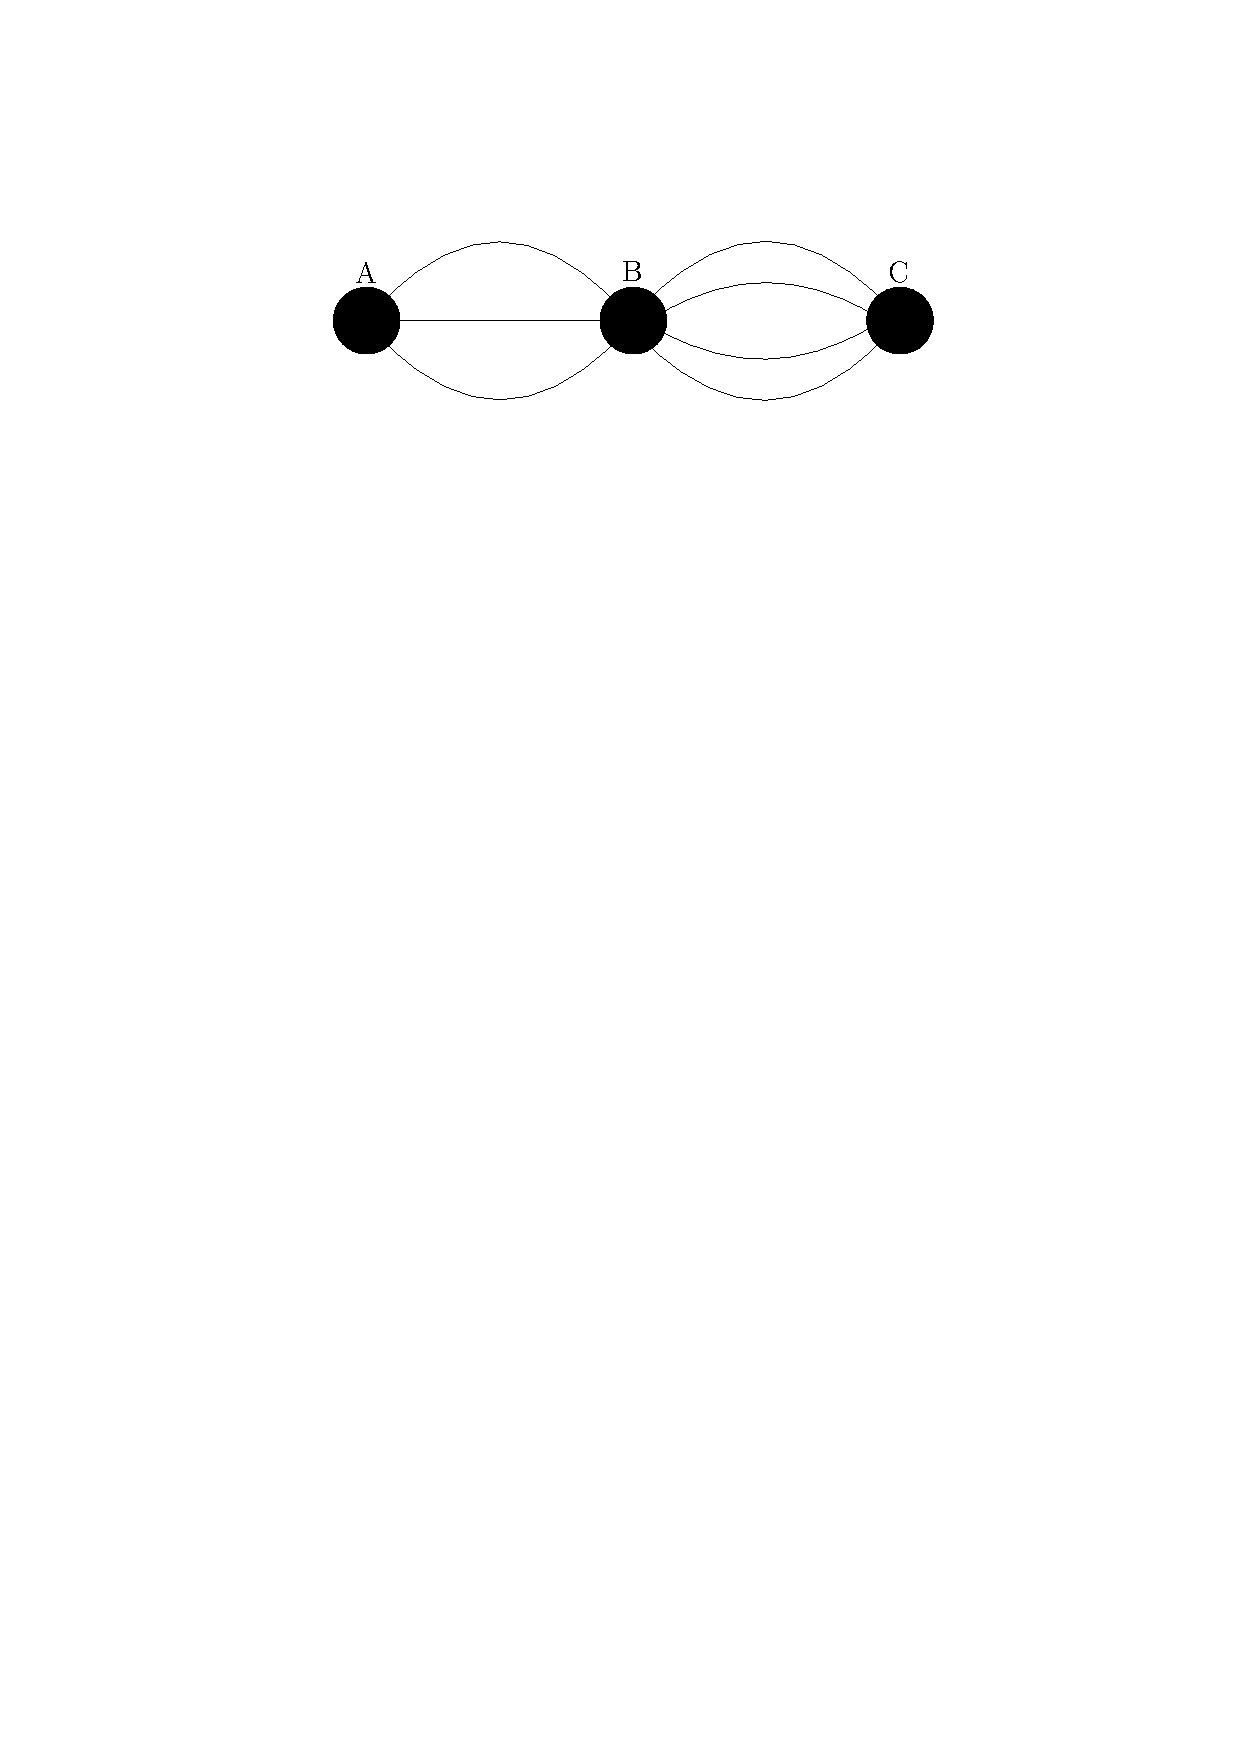
\includegraphics[scale=\normalipe]{ch02_mesta.pdf}
    \caption{Cesty mezi městy $A,\,B,\,C$.}
    \label{fig:mesta}
\end{figure}

Chceme zjistit počet všech způsobů, jak se dostat z města $A$ do města $C$. Jak aplikujeme pravidlo součtu zde? Mohli bychom si zde rozdělit cesty z $A$ do $C$ do množin podle toho, kterou cestou jsme dorazili z $A$ do $B$. Pokud tak učiníme, pak jsme rozdělili cesty do celkem tří množin $P_1,\,P_2,\,P_3$, přičemž všechny jsou po dvou disjunktní (žádná z cest z $A$ do $C$ nemůže obsahovat dvě různé cesty z $A$ do $B$) a množina $P$ obsahuje všechny cesty z $A$ do $C$. Tedy celkový počet cest $\sizeof{P}$ je roven součtu $\sizeof{P_1}+\sizeof{P_2}+\sizeof{P_3}$. Pro každou cestu mezi městy $A$ a $B$ máme 4 možnosti, kudy se dostat z $B$ do $C$. Tedy
\begin{equation*}
    \sizeof{P_1}=\sizeof{P_2}=\sizeof{P_3}=4.
\end{equation*}
To znamená, že celkový počet cest $\sizeof{P}=\sizeof{P_1}+\sizeof{P_2}+\sizeof{P_3}=4+4+4=3\cdot 4=12.$.\par
Tento způsob je jistě velmi nepraktický a navíc je celkem očividné, že na daný výsledek jsme mohli přijít hned. Stačilo vynásobit počet cest mezi městy $A$ a $B$ a počet cest mezi městy $B$ a $C$. Z toho dostáváme druhé kombinatorické pravidlo:

\begin{theorem}[Kombinatorické pravidlo součinu]\label{thm:pravidlo_soucinu}
    Počet uspořádaných $k$-tic, jejichž $i$-tý člen lze vybrat $n_i$ způsoby je roven
    \begin{equation*}
        n_1\cdot n_2\cdot\dots\cdot n_k = \prod_{i=1}^{k}n_i
    \end{equation*}
\end{theorem}
Je důležité zmínit, že jednotlivé výběry \textbf{musí být nezávislé}, tedy výběr na jednu pozici nesmí ovlivnit počet výběrů na ostatní pozice. Méně formálně, avšak užitečněji, můžeme pravidlo formulovat i takto: \textit{Lze-li první výběr provést celkem $n$ způsoby a druhý výběr $m$ způsoby bez ohledu na první výběr, pak celkový počet dvojic možných výběrů je $nm$.} (Pochopitelně, toto lze zobecnit na libovolný počet výběrů, jako je tomu v \ref{thm:pravidlo_soucinu}.)

\begin{exercise}
    Křídy jsou vyráběny
    \begin{itemize}
        \item ve 3 různých barvách,
        \item v 8 různých délkách
        \item a o 4 různých průměrech.
    \end{itemize}
    Kolik typů kříd celkově lze zakoupit? \citep[str. 29]{Brualdi2018}
\end{exercise}
\begin{solution}
    Barvu křídy můžeme vybrat celkem třemi způsoby, délku osmi způsoby a průměr křídy celkem čtyřmi způsoby. Protože výběry jsou na sobě nezávislé, pak podle předchozího pravidla součinu existuje celkem $3\cdot 8\cdot 4=96$ typů kříd.
\end{solution}

\begin{exercise}
    Kolik čtyřciferných přirozených čísel lze sestavit z cifer 0, 1, 2, 3, 4, 5, jestliže
    \begin{enumerate}[label=(\alph*)]
        \item cifry se mohou opakovat,
        \item cifry se nemohou opakovat?
    \end{enumerate}
    (Úloha i řešení \citep[str. 7]{Slavik2022}.)
\end{exercise}
\begin{solution}{Řešení (a)}
    Protože se cifry mohou opakovat, pak na každé číselné pozici máme stejný počet možností výběru číslici, až na první pozici, neboť nemůžeme vybrat číslici 0 (jinak by se nejednalo o \emph{čtyřciferné} číslo). Na první pozici máme tak 5 možností výběru a na zbylých třech máme 6 možností, tj. celkově existuje
    \begin{equation*}
        5\cdot 6\cdot 6\cdot 6 = 1080\;\text{možností.}
    \end{equation*}
\end{solution}
\begin{solution}{Řešení (b)}
    Tentokrát se cifry nesmí opakovat. Úvaha tak zůstává stejná, ale při určování počtu možností výběru musíme zohlednit již vybrané číslice. Na první pozici tak máme 5 možností výběru (nesmíme vybrat nulu), na druhé pozici máme 5 možností (původně jsme měli 6, ale jednu cifru jsme již použili na první pozici), na třetí pozici máme 4 možnosti (2 číslice jsme již použili) a na čtvrté pozici máme 3 možnosti. Celkově tak existuje
    \begin{equation*}
        5\cdot 5\cdot 4\cdot 3=300\;\text{možností.}
    \end{equation*}
\end{solution}

Kombinatorické pravidlo součtu a součinu však můžeme v různých úlohách kombinovat. Speciálně, pokud si tak ulehčíme hledání určených konfigurací.

\begin{exercise}
    Kolik sudých čísel čtyřciferných přirozených čísel lze sestavit z cifer 0, 1, 2, 3, 4, 5, jestliže se nesmí opakovat? (Úloha i řešení \citep[str. 8]{Slavik2022}.)
\end{exercise}
\begin{solution}
    Aby výsledné číslo bylo sudé, musí končit (tj. mít na čtvrté pozici) číslici 0, 2, nebo 4. Zde již však nastává problém, neboť nemůžeme hned aplikovat pravidlo součinu. Je tomu tak proto, že pokud by byla na čtvrté pozici nula, pak na první pozici máme 5 možností, zatímco pokud by zde byla číslice 2, nebo 4, pak počet přípustných číslic na první pozici je již pouze 4 (nesmíme vybrat číslici 0 a pak číslici na čtvrté pozici). Počet výběrů tak již není nezávislý. Nicméně můžeme každý z případů vyšetřit zvlášť:
    \begin{itemize}
        \item označme si množinu $D_1$ (z angl. \emph{digit}) obsahující všechna čísla končící číslicí 0,
        \item množinu čísel $D_2$ končících číslicí 2 a
        \item množinu čísel $D_3$ končících číslicí 4.
    \end{itemize}
    Pro čísla končící nulou máme na první pozici celkem 5 možností, na druhé pak 4 možnosti a na třetí 3 možnosti. Tedy z kombinatorického pravidla součinu máme
    \begin{equation*}
        \sizeof{D_1}=5\cdot 4\cdot 3=60\;\text{možností.}
    \end{equation*}
    Množiny $D_2$ a $D_3$ mají stejnou velikost, neboť v obou případech máme na první pozici 4 možnosti výběru, na druhé 4 možnosti výběru a na třetí 3 možnosti. Tj.
    \begin{equation*}
        \sizeof{D_2}=\sizeof{D_3}=4\cdot 4\cdot 3=48\;\text{možností.}
    \end{equation*}
    Je jasné, že tyto množiny jsou disjunktní (každá dvojice množin obsahuje čísla s jinou číslicí na čtvrté pozici). Tedy podle kombinatorického principu součtu platí
    \begin{equation*}
        \sizeof{D_1\cup D_2\cup D_3}=\sizeof{D_1}+\sizeof{D_2}+\sizeof{D_3}=60+48+48=156\;\text{možností.}
    \end{equation*}
\end{solution}
\section{Variace, permutace a kombinace}

Nyní trochu rozšíříme na repertoár nástrojů. Zatím jsme řešili úlohy, kde jsme vybírali vždy "po jednom" prvku, abychom dosáhli jisté konfigurace. Nyní se podíváme, jakých výsledků dosáhneme v případě, kdy budeme již vybírat nějaké $k$-tice z nějaké $n$ prvkové množiny objektů.\par
Je třeba si rozmyslet dva základní případy:
\begin{itemize}
    \item výběr $k$-tic, kde \textbf{záleží na pořadí},
    \item výběr $k$-tic, kde \textbf{nezáleží na pořadí}.
\end{itemize}
S prvním případem jsme již do jisté míry obeznámeni, neboť u úloh, které jsme řešili, vždy záleželo na pořadí. To tedy vede na sestavování tzv. \emph{uspořádaných $k$-tic}, které jsme již zmínili ve formulaci kombinatorického pravidla součinu \ref{thm:pravidlo_soucinu}. Těm říkáme tzv. \textbf{variace $k$-té třídy z $n$ prvků}. Tedy např. variací 2. třídy z množiny $\set{1,\,2,\,3}$ je třeba
\begin{equation*}
    (1,\,3)\;\;\;\text{nebo}\;\;\;(3,\,1).
\end{equation*}

Druhý případ je pro nás novinkou. Vybíráme totiž tzv. \emph{neuspořádané $k$-tice}, tzn. vybereme-li např. z množiny $\set{a,\,b,\,c}$ neuspořádanou dvojici sestávající z prvků $a$ a $c$, pak je to stejné jako výběr neuspořádané dvojice sestávající z prvků $c$ a $a$. Takový výběr nazýváme \textbf{kombinací $k$-té třídy z $n$ prvků}.

Zatím se omezíme na tzv. variace, resp. kombinace \textbf{bez opakování}.

\subsection{Výběry bez opakování}

Výběrem bez opakování rozumíme výběr $k$-tice prvků takové, že se v ní žádný prvek neopakuje, tzn. každý je v ní nejvýše jednou. Tedy rozlišujeme
\begin{itemize}
    \item \emph{variace bez opakování} a
    \item \emph{kombinace bez opakování}.
\end{itemize}
Pojďme se nyní podívat na metody jejich výpočtu.

\begin{theorem}[Variace bez opakování]\label{thm:variace_bez_opakovani}
    Počet uspořádaných $k$-tic sestavených z $n$-prvkové množiny tak, že se každý prvek ve výběru vyskytne nejvýše jednou, je roven
    \begin{equation*}
        \prod_{i=1}^{k}(n-i+1)=n(n-1)(n-2)\cdots(n-k+1).
    \end{equation*}
\end{theorem}
\begin{proof}
    Tento fakt přímo plyne z kombinatorického pravidla součinu. Na první pozici máme $n$ možností výběru, na druhé $n-1$ možností, \dots a pro $k$-tý člen máme $n-k+1$ možností. Tedy celkově $n(n-1)\cdots(n-k+1)$ možností.
\end{proof}

Počet variací $k$-té třídy z $n$-prvkové množiny bez opakování budeme značit $V_k(n)$.

\begin{exercise}
    Ve třídě, kde je celkem 25 dětí, si žáci volí nového pokladníka, šatnáře a službu na tabuli, přičemž jeden žák nesmí zastávat více pozic zároveň. Kolika různými způsoby si může třída zvolit žáky na dané pozice.
\end{exercise}
\begin{solution}
    V tomto případě jistě záleží na pořadí výběru (vybrat žáka na pozici šatnáře není jistě to samé, jako jej vybrat na pozici pokladníka). Tedy budeme počítat variace 3. třídy z 25 prvků bez opakování, tedy existuje
    \begin{equation*}
        V_3(25)\stackrel{\ref{thm:variace_bez_opakovani}}{=}25\cdot(25-1)\cdot(25-2)=25\cdot 24\cdot 23=13 800\;\text{způsobů.}
    \end{equation*}
\end{solution}

Dalším důležitým, a zatím nezmíněným termínem, je tzv. \emph{permutace}. Permutací rozumíme libovolné uspořádání $n$ prvků do řady. Tedy např. 5, 3, 2, 4, 1 je permutace množiny $\set{1,\,2,\,3,\,4,\,5}$. Permutace lze interpretovat jako uspořádané $n$-tice, což z nich dělá speciální případ variace (výběr uspořádané $n$-tice z $n$ prvkové množiny). Stejně jako u variací a kombinací rozlišujeme permutace s opakováním a bez opakování.
\begin{theorem}[Permutace bez opakování]
    Počet uspořádaných $n$-tic z $n$-prvkové množiny tak, že se každý prvek ve výběru vyskytne nejvýše jednou, je
    \begin{equation*}
        \prod_{i=1}^{n}i=n(n-1)(n-2)\dots 2\cdot 1.
    \end{equation*}
\end{theorem}
\begin{proof}
    Permutace je speciálním případem variace pro $k=n$, tedy $V_n(n)\stackrel{\ref{thm:variace_bez_opakovani}}{=}n(n-1)(n-2)\cdots 2\cdot 1$.
\end{proof}

\begin{definition}[Faktoriál]
    Je-li $n\in\N$, pak definujeme číslo
    \begin{equation*}
        n!=n(n-1)(n-2)\cdots 2\cdot 1=\prod_{i=1}^{n}i,
    \end{equation*}
    které nazýváme \emph{faktoriál} (čteme "$n$ faktoriál").
\end{definition}

Číslo $n!$ tedy vyjadřuje počet permutací $n$ prvkové množiny\footnote{Podobně jako pro variace, i pro permutaci $n$ prvkové množiny se zřídka používá značení $P(n)$. Avšak je tomu tak málokdy, neboť často se při výpočtech píše rovnou $n!$.}.

\begin{exercise}
    Z 10 knih je 6 psáno česky a zbylé 4 latinsky. Kolika různými způsoby lze daná knihy umístit na poličku, jestliže všechny knihy psané česky mají být vedle sebe a všechny latinsky psané vedle sebe?\cite{Havrlant2022}
\end{exercise}
\begin{solution}
    Všechny české knihy chceme seřadit vedle sebe, tj. jedná se o permutaci na šesti prvcích, kterých je $6!$. Podobně latinsky psané knihy lze vedle sebe seřadit $4!$ způsoby. Seřazení český a latinských knih jsou na sobě nezávislá a tedy podle kombinatorického pravidla součinu existuje
    \begin{equation*}
        6!\cdot 4!=(6\cdot 5\cdot 4\cdot 3\cdot 2\cdot 1)\cdot(4\cdot 3\cdot 2\cdot 1)=720\cdot 24=17 280\;\text{možností.}
    \end{equation*}
\end{solution}

Zatím jsme se zabývali uspořádanými $k$-ticemi (variace a permutace), jejichž důležitou vlastností bylo, že záleželo na pořadí. Pokud ovšem chceme od pořadí upustit a soustředit se jen na vybrané prvky, budeme muset náš výpočet lehce upravit.

\begin{theorem}[Kombinace bez opakování]\label{thm:kombinace_bez_opakovani}
    Počet neuspořádaných $k$-tic sestavených z prvků $n$ prvkové množiny tak, že se každý prvek ve výběru vyskytne nejvýše jednou, je roven
    \begin{equation*}
        \dfrac{n(n-1)(n-2)\cdots(n-k+1)}{k!}=\dfrac{1}{k!}\prod_{i=1}^{k}(n-i+1)
    \end{equation*}
\end{theorem}
\begin{proof}
    Naši úvahu můžeme založit na následujícím pozorování: máme-li nějakou \emph{neuspořádanou} $k$-tici prvků z $n$ prvkové množiny, pak existuje přesně $k!$ způsobů, jak vybrané prvky uspořádat do řady, čímž z ní vytvoříme \emph{uspořádanou} $k$-tici. To znamená, že platí
    \begin{equation*}
        (\text{počet uspořádaných $k$-tic})=k!\cdot(\text{počet neuspořádaných $k$-tic}).
    \end{equation*}
    Počet neuspořádaných $k$-tic umíme vypočítat podle věty \ref{thm:variace_bez_opakovani}, tedy máme
    \begin{equation*}
        \prod_{i=1}^{k}(n-i+1)=k!\cdot(\text{počet neuspořádaných $k$-tic}).
    \end{equation*}
    Vydělíme-li rovnost číslem $k!$, dostaneme požadovaný výraz, tj.
    \begin{equation*}
        (\text{počet neuspořádaných $k$-tic})=\dfrac{1}{k!}\prod_{i=1}^{k}(n-i+1)
    \end{equation*}
\end{proof}
\section{Cvičení}

\begin{exercise}\label{exercise:ch02_1}
    \textit{Jana má pět různě barevných triček a tři nestejné sukně. Kolika způsoby si může vzít tričko a sukni, aby pokaždé vypadala jinak?} \citep[str. 145]{Petakova2020}
\end{exercise}
\begin{exercise}\label{exercise:ch02_2}
    V jedné třídě, ve které každý žák ovládá aspoň jeden ze dvou jazyků (angličtinu nebo němčinu), hovoří 25 žáků anglicky, 16 žáků německy a 7 žáků hovoří oběma jazyky. Kolik žáků chodí do této třídy? \citep[sekce Kombinatorika]{kdm2022}
\end{exercise}
\begin{exercise}\label{exercise:ch02_3}
    Určete počet všech přirozených čísel větších než 2000, v jejichž zápisech se vyskytují cifry 1, 2, 4, 6, 8, a to každá nejvýše jednou? \citep[str. 146]{Petakova2020}
\end{exercise}
\begin{exercise}\label{exercise:ch02_4}
    Na běžecké trati běží 8 závodníků. Za předpokladu, že každou z medailí získá právě jeden závodník, vypočítejte, kolik je možností na rozdělení zlaté, stříbrné a bronzové medaile mezi závodníky. \citep[str. 146]{Petakova2020}
\end{exercise}
\begin{exercise}\label{exercise:ch02_5}
    Ve třídě je 30 míst, ale ve třídě 3. B je pouze 28 žáků. Kolika způsoby lze sestavit zasedací pořádek? \citep[str. 146]{Petakova2020}
\end{exercise}
\begin{exercise}\label{exercise:ch02_6}
    Z kolika prvků lze vytvořit 992 variací druhé třídy bez opakování? \citep[str. 146]{Petakova2020}
\end{exercise}
\begin{exercise}\label{exercise:ch02_7}
    Kolika způsoby lze rozmíchat hru 32 karet? \citep[str. 146]{Petakova2020}
\end{exercise}
\begin{exercise}\label{exercise:ch02_8}
    Kolik různých devíticiferných čísel s různými ciframi lze sestavit z cifer 1 až 9? \citep[str. 146]{Petakova2020}
\end{exercise}
\begin{exercise}\label{exercise:ch02_9}
    Kolik přímek určuje deset různých bodů v rovině, z nichž
    \begin{enumerate}[label=(\alph*)]
        \item žádné tři neleží na jedná přímce,
        \item právě šest leží na jedné přímce?
    \end{enumerate}
    \citep[str. 146]{Petakova2020}
\end{exercise}
\begin{exercise}\label{exercise:ch02_10}
    Určete počet všech úhlopříček v konvexním mnohoúhelníku. \citep[str. 147]{Petakova2020}
\end{exercise}
\begin{exercise}\label{exercise:ch02_11}
    V krabici je 10 výrobků, z nichž jsou právě tři vadné. Kolika způsoby lze vybrat 5 výrobků tak, aby:
    \begin{enumerate}[label=(\alph*)]
        \item žádný nebyl vadný,
        \item právě jeden byl vadný,
        \item nejvýše jeden byl vadný,
        \item alespoň dva byly vadné.
    \end{enumerate}
    \citep[str. 147]{Petakova2020}
\end{exercise}
\begin{exercise}\label{exercise:ch02_12}
    Z kolika prvků lze vytvořit 990 kombinací druhé třídy bez opakování? \citep[str. 147]{Petakova2020}
\end{exercise}
\begin{exercise}\label{exercise:ch02_13}
    Učitel chce vytvořit ze čtyř dívek a čtyř chlapců jeden tříčlenný tým, v němž bude jedna dívka a dva chlapci. Kolika různými způsoby může sestavit tým? \citep[příklad \emph{Tříčlenné 69274}]{hackmath2022}
\end{exercise}
    \chapter{Kombinatorické identity}

Nyní jsme si již prošli základní nástroje, které v kombinatorice využíváme. V rámci minulé kapitoly jsme si ukázali práci s kombinačními čísly a především jejich význam. Nyní se na ně trochu více zaměříme, neboť zjistíme, že tento matematický objekt má pozoruhodné vlastnosti, díky kterým obdržíme několik zajímavých identit.

\section{Vlastnosti kombinačních čísel}

V této sekci se budeme \emph{především} (avšak ne vždy) držet naší původní definice kombinačního čísla z \ref{def:kombinacni_cislo}, tj.
\[\binom{n}{k}=\dfrac{n(n-1)(n-2)\cdots(n-k+1)}{k!},\]
a to právě kvůli již zmíněné vlastnosti, že oproti
\[\dfrac{n!}{(n-k)!k!}\]
dává výraz smysl i pro $k>n$ a je vždy roven nule (ostatně i z kombinatorického hlediska dává tento výsledek smysl). Nebudeme se tak muset explicitně odvolávat na předpoklad, že $n\leqslant k$, abychom předešli formálním nepřesnostem.
\medskip

U kombinačních čísel lze pozorovat některé zajímavé vlastnosti. Začneme asi tou nejzákladnější.
\begin{theorem}[Symetrie kombinačních čísel]
    Pro $n,\,k\in\N_0$, kde $k\leqslant n$, platí
    \[\binom{n}{k}=\binom{n}{n-k}.\]
\end{theorem}
\begin{proof}[Důkaz první]
    Asi nejjednodušší důkaz je přímým výpočtem:
    \[\binom{n}{n-k}=\dfrac{n!}{(n-(n-k))(n-k)!}=\dfrac{n!}{k!(n-k)!}=\binom{n}{k}.\]
\end{proof}
\begin{proof}[Důkaz druhý]
    Názornější důkaz nám poskytne kombinatorická interpretace tohoto tvrzení. Libovolná $k$-tice (v tomto smyslu množina) je jednoznačně určena výběrem prvků z nějaké $n$ prvkové množiny, které jí budou náležet. Výběrem $k$ prvků z dané množiny tak zbude $n-k$ prvků, které nejsou součástí dané $k$-tice.
    \todo{obrázek}
\end{proof}
\section{Binomická věta}

Kombinační čísla mají kromě kombinatorických úloh využití i v klasické aritmetice. Ať už se to zdá, nebo ne, tyto dva možná zdánlivě rozdílné světy si nejsou až tak vzdálené. V této sekci se proto podíváme na větu, která nám trochu více zobecní koncept roznásobování dvojčlenů.\par
Podívejme se nejdříve na ty nejjednodušší případy:
\begin{align*}
    (x+y)^0&=1,\\
    (x+y)^1&=x+y,\\
    (x+y)^2&=x^2+2xy+y^2,\\
    (x+y)^3&=x^3+3x^2y+3xy^2+y^3,\\
    (x+y)^4&=x^4+4x^3y+6x^2y^2+4xy^3+y^4,\\
    &\vdots
\end{align*}
Čeho bychom si mohli na poprvé možná všimnout je faktu, že koeficienty u jednotlivých členů jsou symetrické. To je asi nejlépe vidět u roznásobení čtvrté mocniny dvojčlenu $x+y$. Proč tomu ale tak je? Vzpomeňme si na větu \ref{thm:symetrie_kombinacnich_cisel}, díky které jsme se dozvěděli, že kombinační čísla jsou "symetrická", tzn. $\binom{n}{k}=\binom{n}{n-k}$. Další pozorování bychom z tohoto zápisu učili nejspíše stěží (avšak klobouček dolů všem, kteří to již vidí :-)). Zkusme se zaměřit nyní čistě na dané koeficienty. Počet členů je vždy totiž lichý, což nám umožňuje zapsat si jejich koeficienty ve schématu níže.
\begin{figure}[H]
    \centering
    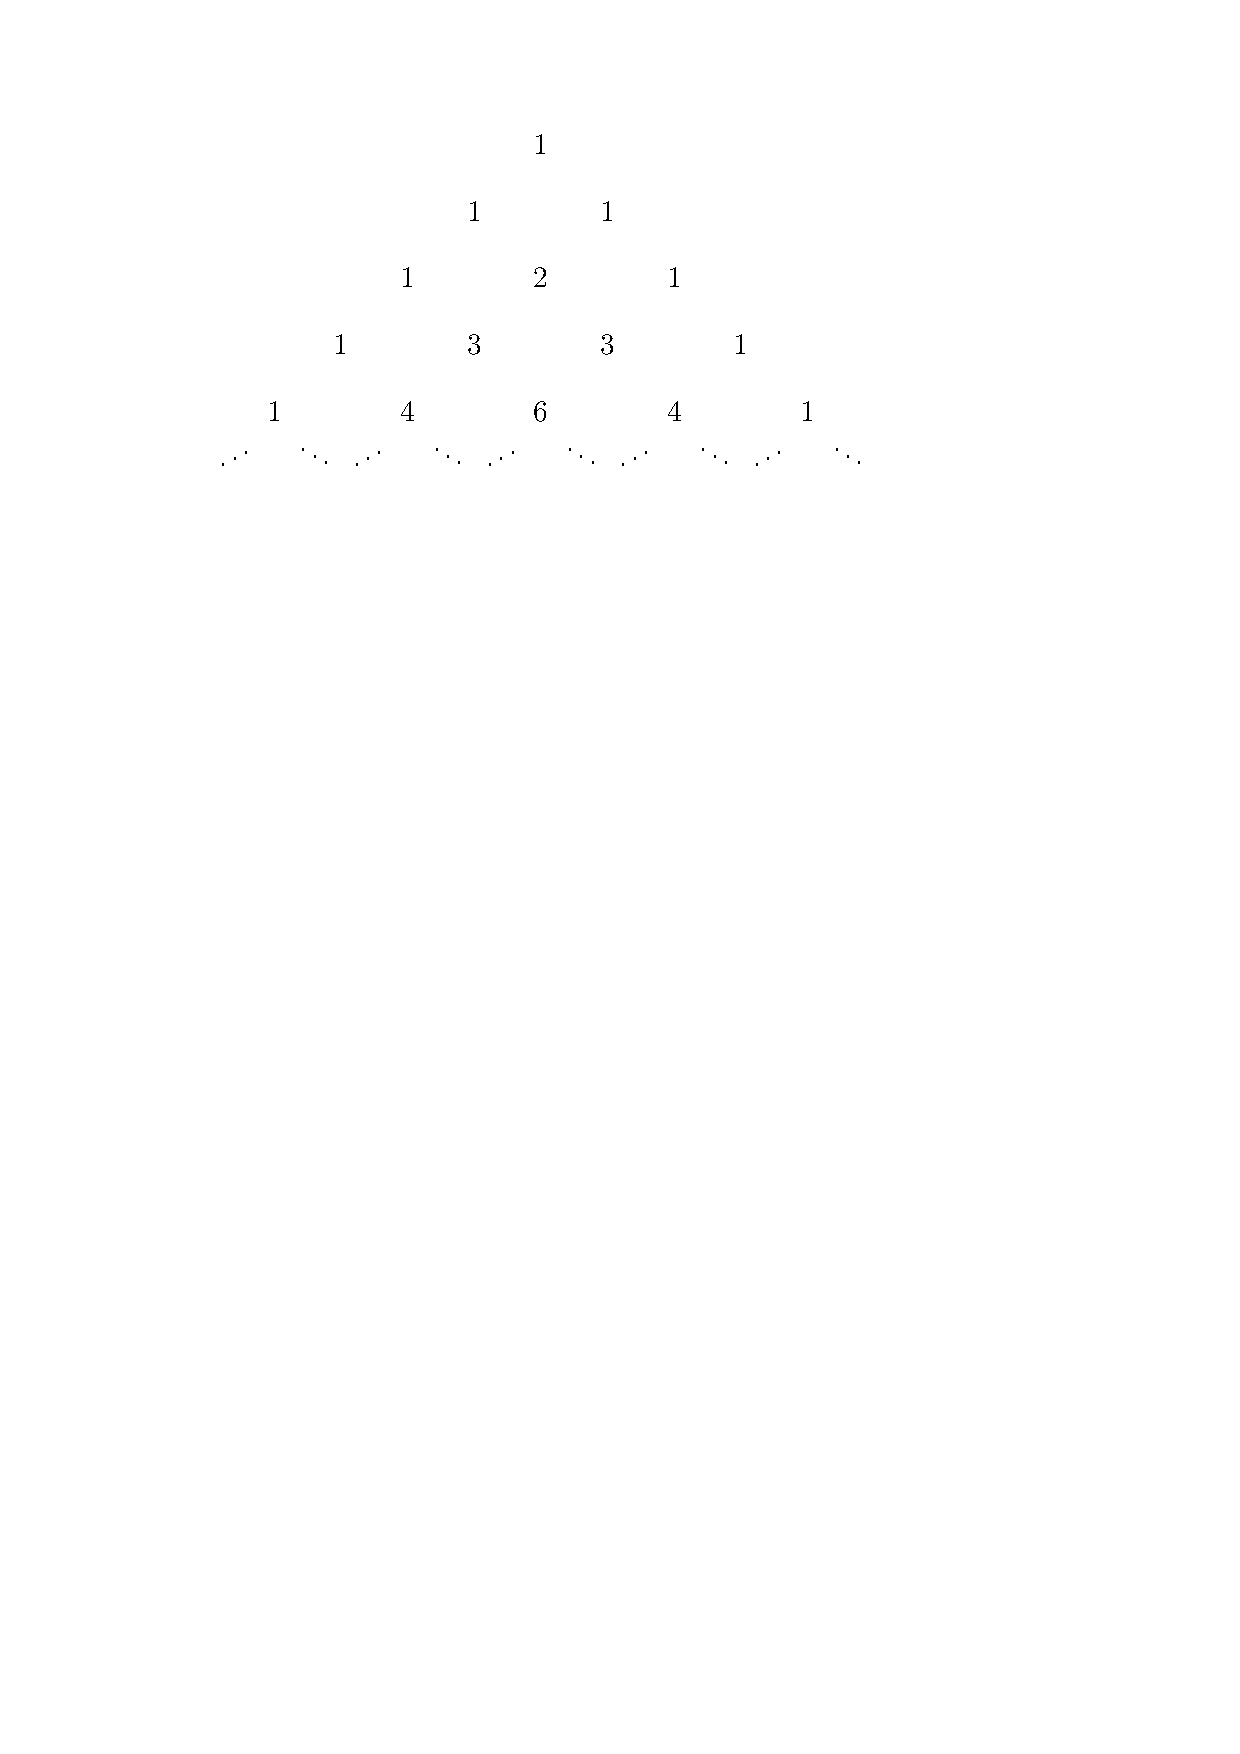
\includegraphics[scale=\normalipe]{ch03_pascaluv_trojuhelnik.pdf}
    \caption{Schéma koeficientů ve tvaru pyramidy.}
    \label{fig:pascaluv_trojuhelnik}
\end{figure}
Toto schéma se nazývá \textbf{Pascalův trojúhelník}. Pokud se podíváme blíže, lze si všimnout, jak vznikají jeho řádky. Na kraji vždy pevně stojí číslo 1 a další koeficienty vzniknou součtem koeficientů nad ním.
\begin{figure}[H]
    \centering
    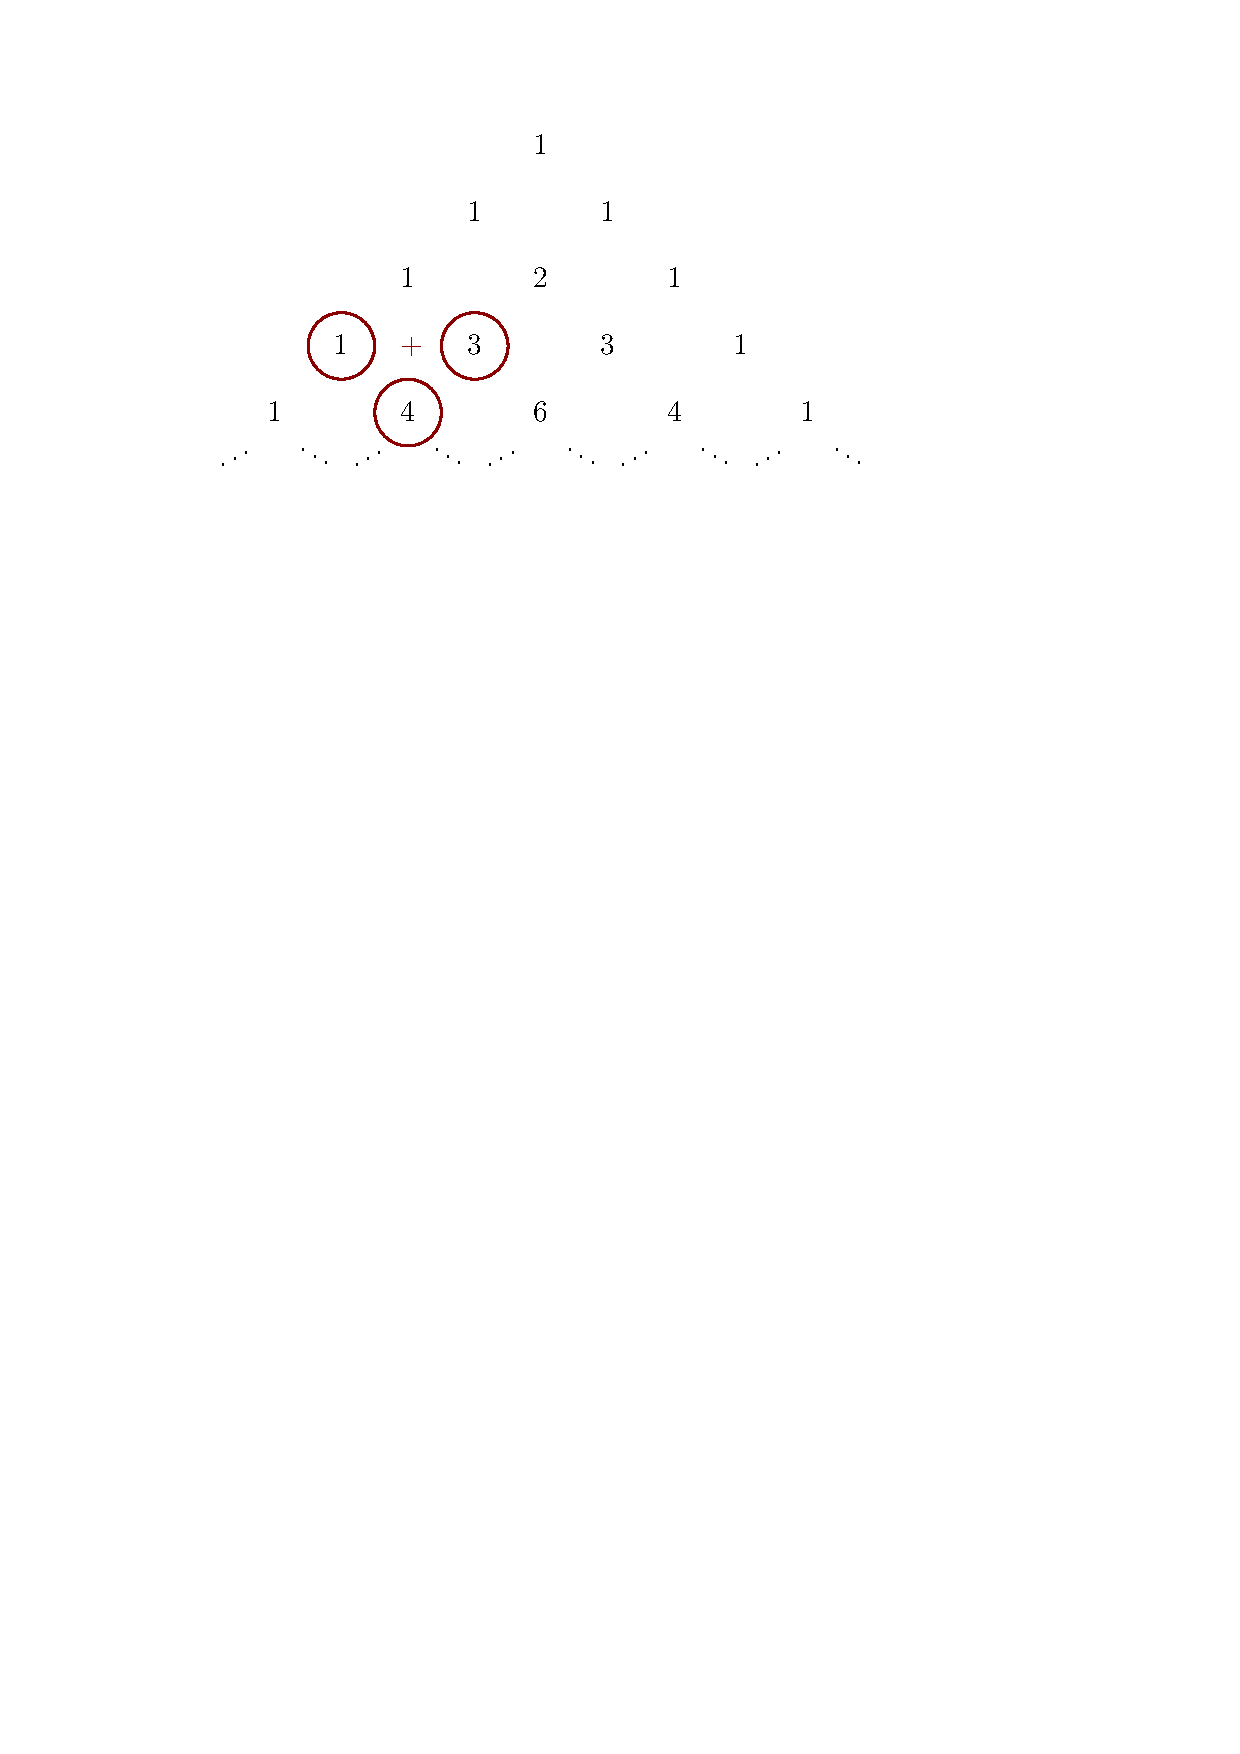
\includegraphics[scale=\normalipe]{ch03_pascaluv_trojuhelnik_soucet.pdf}
    \caption{Generování Pascalova trojúhelníku součtem členů.}
    \label{fig:pascaluv_trojuhelnik_soucet}
\end{figure}
Pokud se nyní vrátíme opět ke kombinačním číslům, jistě si vzpomeneme, že jsme zde měli větu \ref{thm:soucet_kombinacnich_cisel}, která dávala do souvislosti kombinační čísla a jejich součet. Z toho by nás tak mohlo napadnout, že jednotlivá čísla v Pascalově trojúhelníku by tak mohla odpovídat jistým kombinačním číslům. Je tomu skutečně tak.
\begin{figure}[H]
    \centering
    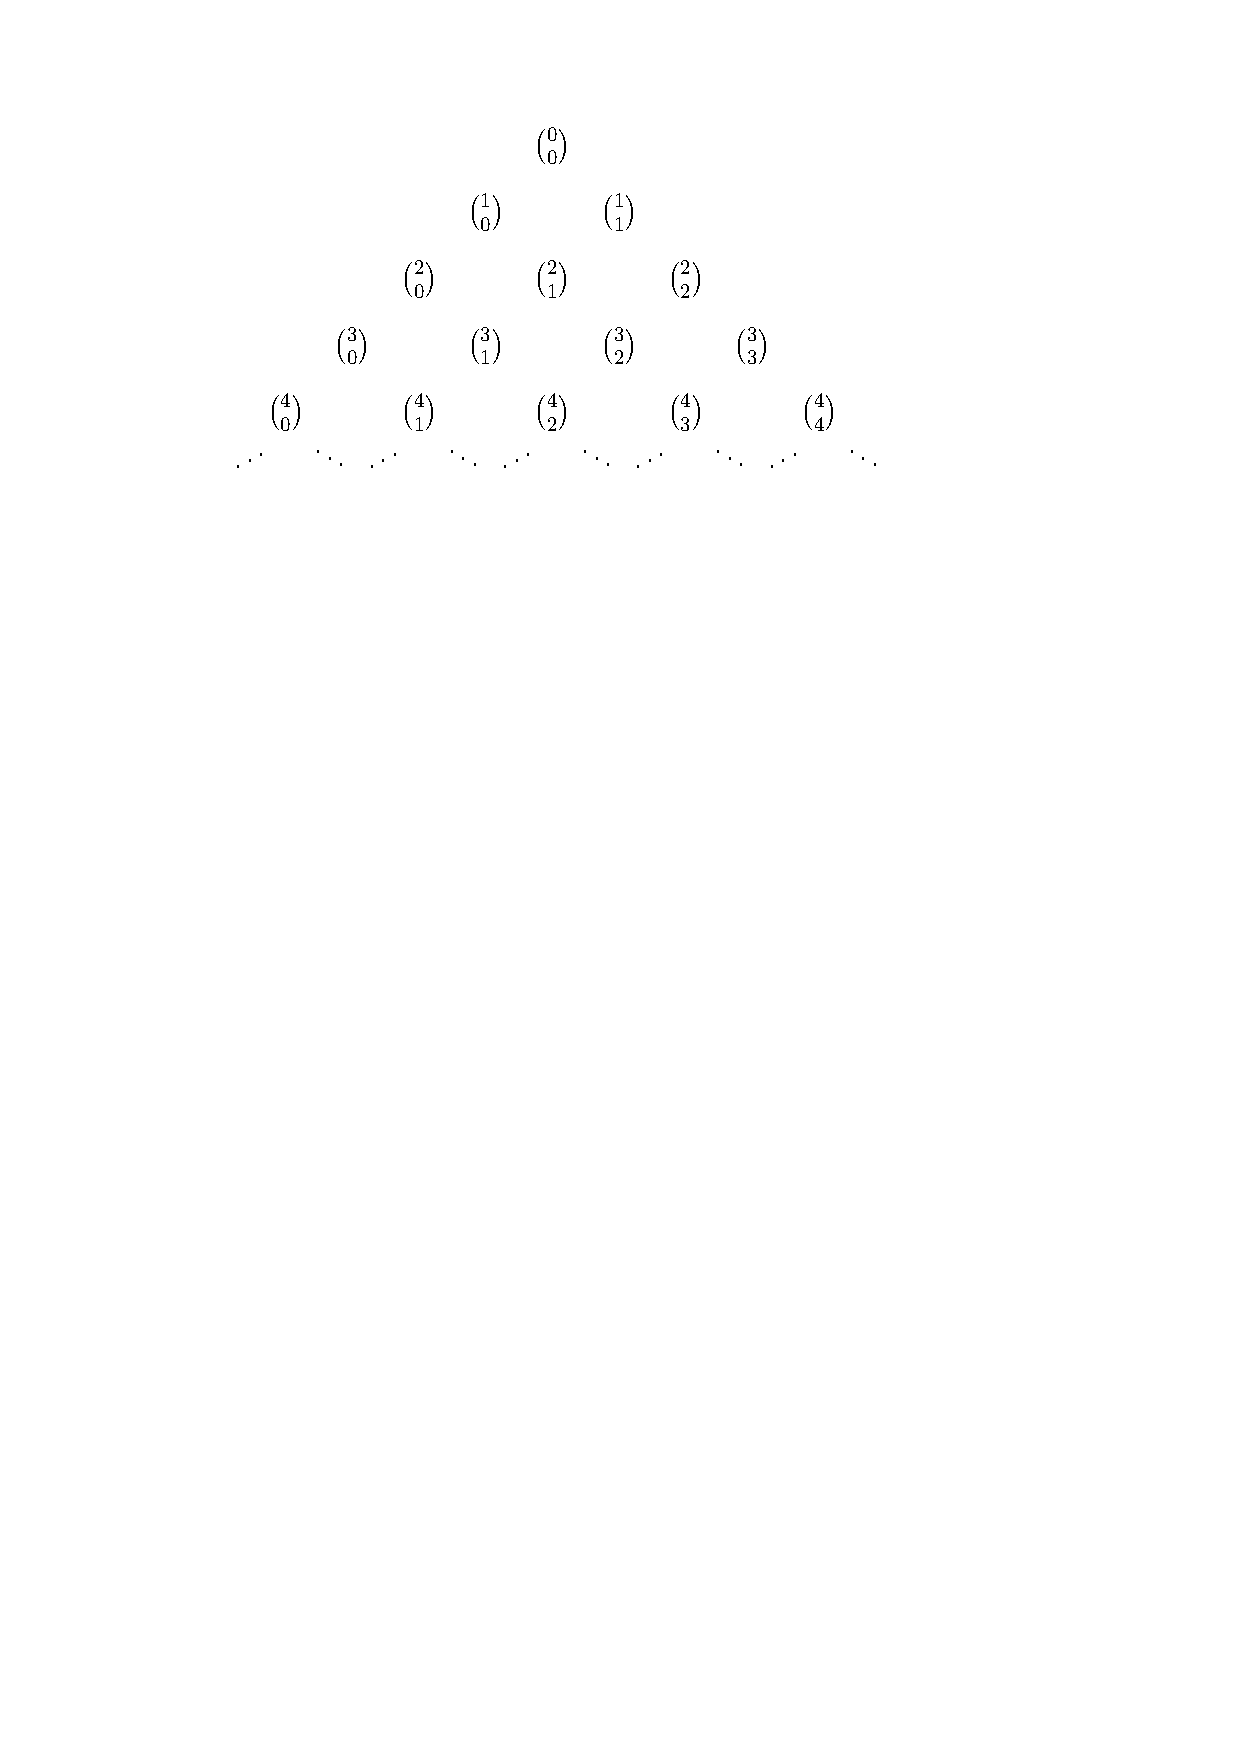
\includegraphics[scale=\normalipe]{ch03_pascaluv_trojuhelnik_kombinacni_cisla.pdf}
    \caption{Pascalův trojúhelník pomocí kombinačních čísel.}
    \label{fig:pascaluv_trojuhelnik_kombinacni_cisla}
\end{figure}
Sami se můžete přesvědčit, že jednotlivá kombinační čísla odpovídají daným koeficientům. Navíc zde lze i vidět i jejich další vlastnosti v uplatnění, konkrétně věty \ref{thm:symetrie_kombinacnich_cisel} (stačí se podívat na $k$-tý člen a příslušném $(n-k)$-tý člen, kde $n$ zde představuje číslo řádku od nuly, neboť odpovídá mocnině daném dvojčlenu) a \ref{thm:soucet_kombinacnich_cisel} (koeficient různý od jedničky na kraji je součtem koeficientů nad ním).\par

Vraťme se nyní k roznásobování dvojčlenů. Z Pascalova trojúhelníku lze tak vidět, že koeficienty v rozvoji $(x+y)^n$ by mohly být po řadě čísla
\[\binom{n}{0},\,\binom{n}{1},\,\binom{n}{2},\,\cdots,\,\binom{n}{n}.\]
Jak lze ukázat, platí totiž následující věta.
\begin{theorem}[Binomická]\label{thm:binomicka_veta}
    Pro libovolná $x,\,y\in\C$ a $n\in\N$ platí
    \[(x+y)^n=\sum_{k=0}^{n}\binom{n}{k}x^{n-k}y^k,\]
    neboli
    \[(x+y)^n=\binom{n}{0}x^ny^0+\binom{n}{1}x^{n-1}y^1+\binom{n}{2}x^{n-2}y^2+\cdots+\binom{n}{n}x^0y^n.\]
\end{theorem}
\begin{proof}
    Nejnázornějším důkazem pro nás opět bude kombinatorická úvaha. Rozepišme si součin $(x+y)^n$ jako
    \[\underbrace{(x+y)(x+y)\cdots(x+y)}_{n\text{-krát}}.\]
    Sečíst můžeme pouze členy, které mají v součinu stejný počet $x$ a stejný počet $y$. Např.
    \[(x+y)(x+y)(x+y)=xxx+xxy+xyx+yxx+xyy+yxy+yyx+yyy=x^3+3x^2y+3xy^2+y^3.\]
    Člen $x^{n-k}y^k$ tvoří tak uspořádanou $n$-tici činitelů z $x$ a $y$.
    \[\underbrace{x\cdot x\cdots x}_{(n-k)\text{-krát}} \cdot \underbrace{y\cdot y\cdots y}_{k\text{-krát}}.\]
    Takovou uspořádanou $n$-tici můžeme sestavit tak, že vybereme $k$ pozic pro činitel $y$ (zbylých $n-k$ pozic doplníme činitelem $x$). Takových výběrů existuje $\binom{n}{k}$, a tedy v tomto počtu se daný člen objeví v rozvoji $(x+y)^n$.
\end{proof}
\begin{task}
    Vypočítejte rozvoj $\displaystyle \left(x+\dfrac{1}{2y}\right)^5$.
\end{task}
\begin{solution}
    Postupujeme podle binomické věty \ref{thm:binomicka_veta}:
    \begin{align*}
        \left(x+\dfrac{1}{2y}\right)^5 &\stackrel{\ref{thm:binomicka_veta}}{=}\sum_{k=0}^{5}\binom{5}{k}x^{5-k}\left(\dfrac{1}{2y}\right)^k \\
        &=\binom{5}{0}x^5\left(\dfrac{1}{2y}\right)^0+\binom{5}{1}x^4\left(\dfrac{1}{2y}\right)^1+\binom{5}{2}x^3\left(\dfrac{1}{2y}\right)^2+\binom{5}{3}x^2\left(\dfrac{1}{2y}\right)^3\\ &+\binom{5}{4}x^1\left(\dfrac{1}{2y}\right)^4+\binom{5}{5}x^0\left(\dfrac{1}{2y}\right)^5\\
        &=x^5+5\cdot\dfrac{x^4}{2y}+10\cdot\dfrac{x^3}{4y^2}+10\cdot\dfrac{x^2}{8y^3}+5\cdot\dfrac{x}{16y^4}+\dfrac{1}{32y^5}.
    \end{align*}
\end{solution}
\begin{task}
    Vypočítejte desátý člen rozvoje $(a+2b)^{15}$.
\end{task}
\begin{solution}
    Pochopitelně bychom zde mohli vypočítat celý rozvoj a podívat se na jeho patnáctý člen, nicméně díky binomické větě známe tvar každého členu.
    \[(a+2b)^15=\sum_{k=0}^{15}\binom{15}{k}a^{15-k}(2b)^k\]
    Desátý člen vypočítáme pro $k=9$ (rozvoj začíná od $k=0$):
    \[\binom{15}{9}a^{15-9}(2b)^{9}=5005\cdot a^6\cdot 512b^9=2\,562\,560a^6b^9.\]
\end{solution}

Pojďme se nyní podívat na některé další kombinatorické identity.
\begin{theorem}\label{thm:vsechny_podmnoziny}
    Pro všechna $n\in\N$ platí
    \[\sum_{k=0}^{n}\binom{n}{k}=2^n,\]
    neboli
    \[\binom{n}{0}+\binom{n}{1}+\cdots+\binom{n}{n}=2^n.\]
\end{theorem}
\begin{proof}[Důkaz první]
    Tvrzení přímo plyne z binomické věty, dosadíme-li $a=b=1$, tj.
    \[\sum_{k=0}^{n}\binom{n}{k}=\sum_{k=0}^{n}\binom{n}{k}1^{n-k}1^k\stackrel{\ref{thm:binomicka_veta}}{=}(1+1)^n=2^n.\]
\end{proof}
\begin{proof}[Důkaz druhý]
    Rovnost lze zdůvodnit opět i kombinatoricky. Pravá strana vyjadřuje počet všech možných neuspořádaných výběrů (libovolné velikosti, tj. pro $k=0,\,\dots,\,n$) z $n$-prvkové množiny. Počet takových výběrů jednoduše odpovídá součtu počtů všech výběrů $k$-tic přes všechny velikosti (tj. přes všechna $k$), tzn.
    \[\binom{n}{0}+\binom{n}{1}+\cdots+\binom{n}{n}.\]
    Libovolnou $k$-tici lze však také vybrat tak, že pro každý z prvků dané množiny nezávisle určíme, zda bude náležet dané $k$-tici, či nebude. Pro každý prvek tak máme 2 možnosti výběru, tj.
    \[\underbrace{2\cdot 2\cdots 2}_{n\text{-krát}}=2^n.\]
\end{proof}
\begin{task}
    Ve firmě pracuje celkem 100 zaměstnanců. Kolika způsoby lze vybrat skupinu zaměstnanců, kteří budou pracovat na technickém oddělení a jednoho z nich zvolit jako vedoucího?
\end{task}
\begin{solution}
    Protože nemáme pevně zadané množství zaměstnanců, kteří budou na oddělení pracovat, pak uvažujeme skupiny všech možných velikostí. Nejdříve vybereme vedoucího a následně k němu přidáme skupinu ze zbývajících $n-1$ zaměstnanců. Vedoucího můžeme vybrat celkem $n$ způsoby. Ze zbylých $n-1$ zaměstnanců lze utvořit skupinu celkem $\sum_{k=0}^{n-1}\binom{n-1}{k}$ způsoby, což je podle předchozí věty \ref{thm:vsechny_podmnoziny} rovno $2^{n-1}$. Celkově lze tedy vybrat skupinu zaměstnanců na dané oddělení $n\cdot 2^{n-1}$ způsoby.
\end{solution}
\begin{theorem}
    Počet neuspořádaných výběrů z $n$-prvkové množiny se sudým počtem prvků je stejný jako počet neuspořádaných výběrů z $n$-prvkové množiny s lichým počtem prvků.
\end{theorem}
\begin{proof}[Důkaz první]
    K důkazu lze opět využít binomickou větu. Začneme tím, že si trochu netradičně zapíšeme nulu:
    \[0=1-1=(1-1)^n=(1+(-1))^n,\]
    což je podle binomické věty rovno
    \[\sum_{k=0}^{n}\binom{n}{k}1^{n-k}(-1)^k=\sum_{k=0}^{n}(-1)^k\binom{n}{k}.\]
    Tento součet si však můžeme rozdělit na dvě sumy podle toho, zda je $k$ sudé nebo liché:
    \[\sum_{k=0}^{n}(-1)^k\binom{n}{k}=\sum_{\substack{0\,\leqslant\,k\,\leqslant\,n \\ k\,\text{sudé}}}(-1)^k\binom{n}{k}+\sum_{\substack{0\,\leqslant\,k\,\leqslant\,n \\ k\,\text{liché}}}(-1)^k\binom{n}{k}=\sum_{\substack{0\,\leqslant\,k\,\leqslant\,n \\ k\,\text{sudé}}}\binom{n}{k}-\sum_{\substack{0\,\leqslant\,k\,\leqslant\,n \\ k\,\text{liché}}}\binom{n}{k}.\]
    U první sumy, kde $k$ je sudé, je výraz $(-1)^k$ vždy roven jedné a u druhé sumy, kde $k$ je liché je naopak $(-1)^k$ vždy rovno $-1$, přičemž toto číslo jsme vytkli z celé sumy. Na začátku jsme však začínali s nulou a tedy platí
    \[\sum_{\substack{0\,\leqslant\,k\,\leqslant\,n \\ k\,\text{sudé}}}\binom{n}{k}-\sum_{\substack{0\,\leqslant\,k\,\leqslant\,n \\ k\,\text{liché}}}\binom{n}{k}=0.\]
    Přičtením druhé sumy k celé rovnosti, tj.
    \[\sum_{\substack{0\,\leqslant\,k\,\leqslant\,n \\ k\,\text{liché}}}\binom{n}{k},\]
    dostaneme
    \[\sum_{\substack{0\,\leqslant\,k\,\leqslant\,n \\ k\,\text{sudé}}}\binom{n}{k}=\sum_{\substack{0\,\leqslant\,k\,\leqslant\,n \\ k\,\text{liché}}}\binom{n}{k}\]
    neboli
    \[\binom{n}{0}+\binom{n}{2}+\binom{n}{4}+\cdots=\binom{n}{1}+\binom{n}{3}+\binom{n}{5}+\cdots\]
    Kombinatoricky obě strany rovnosti vyjadřují počty výběrů z $n$ prvkové množiny se sudým, resp. lichým počtem prvků. Protože jsou si však tyto počty rovny, dostáváme tvrzení věty.
\end{proof}
\begin{proof}[Důkaz druhý]
    Rovnost lze také zdůvodnit kombinatoricky. Uvažme, že provádíme výběr z množiny $\set{1,\,\dots,\,n}$. Dále uvažujme následující operace: pokud vybraná množina prvků obsahuje číslo 1, pak jej z množiny odstraníme a naopak pokud vybraná množina neobsahuje číslo 1, pak jej do množiny přidáme. V obou případech se tak vždy změní počet prvků o jeden, tedy z výběru sudé velikosti se stane výběr liché velikosti a naopak. Každý výběr sudé velikosti tak lze "spárovat" s výběrem liché velikosti a tedy výběrů obou typů musí být stejně mnoho.
\end{proof}

Poslední, co si zde zmíníme, je tzv. \emph{Vandermondova identita} (též \emph{konvoluce}), kterou později využijeme.
\begin{theorem}[Vandermondova identita]\label{thm:vandermondova_identita}
    Pro všechna $n,\,m,\,r\in\N_0$ platí
    \[\sum_{k=0}^{r}\binom{n}{k}\binom{m}{r-k}=\binom{n+m}{r}.\]
\end{theorem}
\begin{proof}
    Důkaz lze provést (jako u všech ostatních vztahů) výpočtem, ale zde si vystačíme s kombinatorickou interpretací. Představme si, že máme komisi sestávající z $m$ mužů a $n$ žen. Pravá strana udává počet všech možných $r$-tic, které lze vybrat z komise. Těch je $\binom{n+m}{r}$. Obecný sčítanec $\binom{n}{k}\binom{m}{r-k}$ na pravé straně udává počet všech $r$-tic s právě $k$ ženami a $r-k$ muži. Součtem přes všechna $k$ musíme obdržet počet všech možných $r$-tic.
\end{proof}
\section{Cvičení}

\begin{exercise}\label{exercise:ch02_1}
    \textit{Jana má pět různě barevných triček a tři nestejné sukně. Kolika způsoby si může vzít tričko a sukni, aby pokaždé vypadala jinak?} \citep[str. 145]{Petakova2020}
\end{exercise}
\begin{exercise}\label{exercise:ch02_2}
    V jedné třídě, ve které každý žák ovládá aspoň jeden ze dvou jazyků (angličtinu nebo němčinu), hovoří 25 žáků anglicky, 16 žáků německy a 7 žáků hovoří oběma jazyky. Kolik žáků chodí do této třídy? \citep[sekce Kombinatorika]{kdm2022}
\end{exercise}
\begin{exercise}\label{exercise:ch02_3}
    Určete počet všech přirozených čísel větších než 2000, v jejichž zápisech se vyskytují cifry 1, 2, 4, 6, 8, a to každá nejvýše jednou? \citep[str. 146]{Petakova2020}
\end{exercise}
\begin{exercise}\label{exercise:ch02_4}
    Na běžecké trati běží 8 závodníků. Za předpokladu, že každou z medailí získá právě jeden závodník, vypočítejte, kolik je možností na rozdělení zlaté, stříbrné a bronzové medaile mezi závodníky. \citep[str. 146]{Petakova2020}
\end{exercise}
\begin{exercise}\label{exercise:ch02_5}
    Ve třídě je 30 míst, ale ve třídě 3. B je pouze 28 žáků. Kolika způsoby lze sestavit zasedací pořádek? \citep[str. 146]{Petakova2020}
\end{exercise}
\begin{exercise}\label{exercise:ch02_6}
    Z kolika prvků lze vytvořit 992 variací druhé třídy bez opakování? \citep[str. 146]{Petakova2020}
\end{exercise}
\begin{exercise}\label{exercise:ch02_7}
    Kolika způsoby lze rozmíchat hru 32 karet? \citep[str. 146]{Petakova2020}
\end{exercise}
\begin{exercise}\label{exercise:ch02_8}
    Kolik různých devíticiferných čísel s různými ciframi lze sestavit z cifer 1 až 9? \citep[str. 146]{Petakova2020}
\end{exercise}
\begin{exercise}\label{exercise:ch02_9}
    Kolik přímek určuje deset různých bodů v rovině, z nichž
    \begin{enumerate}[label=(\alph*)]
        \item žádné tři neleží na jedná přímce,
        \item právě šest leží na jedné přímce?
    \end{enumerate}
    \citep[str. 146]{Petakova2020}
\end{exercise}
\begin{exercise}\label{exercise:ch02_10}
    Určete počet všech úhlopříček v konvexním mnohoúhelníku. \citep[str. 147]{Petakova2020}
\end{exercise}
\begin{exercise}\label{exercise:ch02_11}
    V krabici je 10 výrobků, z nichž jsou právě tři vadné. Kolika způsoby lze vybrat 5 výrobků tak, aby:
    \begin{enumerate}[label=(\alph*)]
        \item žádný nebyl vadný,
        \item právě jeden byl vadný,
        \item nejvýše jeden byl vadný,
        \item alespoň dva byly vadné.
    \end{enumerate}
    \citep[str. 147]{Petakova2020}
\end{exercise}
\begin{exercise}\label{exercise:ch02_12}
    Z kolika prvků lze vytvořit 990 kombinací druhé třídy bez opakování? \citep[str. 147]{Petakova2020}
\end{exercise}
\begin{exercise}\label{exercise:ch02_13}
    Učitel chce vytvořit ze čtyř dívek a čtyř chlapců jeden tříčlenný tým, v němž bude jedna dívka a dva chlapci. Kolika různými způsoby může sestavit tým? \citep[příklad \emph{Tříčlenné 69274}]{hackmath2022}
\end{exercise}
    \chapter{Základy teorie pravděpodobnosti}

\section{Co je to pravděpodobnost?}

\textbf{Pravděpodobnost} (někdy též \emph{šance}) je jeden z pojmů, který vystupuje nejen v matematice, ale i v reálném životě. Když si hodíme mincí, asi je nám jasné, že je stejná šance, že nám padne rub nebo líc. Naopak třeba u hodu klasicky hrací kostkou máme šanci $1:6$, že nám padne jednička a šance tak již není vyrovnaná situaci, že nám nepadne. Intuitivně tak asi tušíme, co se myslí, když se řekne, že např. šance výhry je 75 \%. Co však ale reprezentuje ono číslo? Definovat, co je to "skutečná" pravděpodobnost je obtížné a jedná se spíše o záležitost filozofickou. V matematice se však tomuto problému dokážeme vyhnout.\par
Jako lidé chápeme, že šance výhry 70 \% je v jistém smyslu "lepší" než např. 30 \%, ale proč tomu tak je? Pro příklad si vezměme již zmíněnou klasickou hrací kostku. Pro simulaci hodů využijeme jednoduchý program v jazyce Python:
\VerbatimInput{components/chapter04/sections/dice.py}

Níže je tabulka četností výskytů a jejich poměru vůči celkovému počtu jednotlivých ok po miliónu pokusů.
\begin{table}[H]
    \centering
    \begin{tabular}{|c|c|c|}
    \hline
    Počet ok & Četnost & Výskyt (\%)     \\ \hline
    1     & 166 896 & $16{,}6896$ \\
    2     & 166 789 & $16{,}6789$ \\
    3     & 166 508 & $16{,}6508$ \\
    4     & 166 863 & $16{,}6863$ \\
    5     & 166 151 & $16{,}6150$ \\
    6     & 166 794 & $16{,}6794$ \\ \hline
    \end{tabular}
    \caption {Četnost hodů ok na hrací kostce po miliónu pokusech.}
\end{table}
Víme, že šance pro všechny strany je stejná - $1:6$, což odpovídá hodnotě numerické hodnotě $0{,}1\overline{6}$, neboli $16{,}\overline{6}$. Celkově tak můžeme vidět, že procentuální výskyt se jen málo liší od našeho očekávání. Tímto způsobem můžeme vnímat pravděpodobnost. Jako číslo ke kterému se blíží \textbf{poměr počtu příznivých pokusů a počtu všech pokusů}.\par
Praktický výpočet pravděpodobnosti však probíhá trochu jinak. U kostky jsme určili pravděpodobnost hodu jedničky tak, že jsme vzali \textbf{počet příznivých hodů} ku \textbf{počtu všech možných hodů}. A v tomto duchu také definujeme pravděpodobnost.\par
\begin{definition}[Elementární a náhodný jev, pravděpodobnost]\label{def:elementarni_nahodny_jev_pravdepodobnost}
    Mějme množinu $\Omega=\set{\omega_1,\,\omega_2,\,\dots,\,\omega_n}$. Pak
    \begin{itemize}
        \item $\Omega$ nazýváme \textbf{množinou elementárních jevů} a libovolný její prvek $\omega_i$ \textbf{elementárním jevem}.
        \item libovolnou podmnožinu $A\subseteq\Omega$ nazýváme \textbf{(náhodný) jev}.
    \end{itemize}
    Dále definujeme funkci $\Prob$ přiřazující libovolnému jevu $A\subseteq\Omega$ reálné číslo z intervalu $\langle0,\,1\rangle$ splňující
    \begin{enumerate}[label=(\roman*)]
        \item $\Prob(\emptyset)=0$,
        \item $\Prob(\Omega)=1$,
        \item $\Prob(A\cup B)=\Prob(A)+\Prob(B)$,
    \end{enumerate}
    kde $A,\,B\subseteq\Omega$ jsou disjunktní jevy. Číslo $\Prob(A)$ nazýváme \textbf{pravděpodobností jevu $A$}.
\end{definition}
Poslední vztah lze zobecnit pro obecný počet disjunktních jevů $A_1,\,A_2,\,\dots,\,A_n$, tj.
\[\Prob\left(\bigcup\limits_{i=1}^{n}A_i\right)=\sum_{i=1}^{n}\Prob(A_i).\]
Ve všech příkladech dále budeme pracovat s variantou, že všechny elementární jevy jsou stejně pravděpodobné. To má tedy za následek způsob výpočtu, který jsme zmínili výše, tedy je-li $A\subseteq\Omega$ libovolný jev, pak pravděpodobnost jevu $A$ stanovíme jako
\[\Prob(A)=\dfrac{\sizeof{A}}{\sizeof{\Omega}}.\]
\begin{example}
    V případě hodu kostkou tvoří množinu elementárních jevů $\Omega$ případy, kdy 1 až 6 ok. Označíme-li si jednotlivé počty ok $O_1,\,\dots,\,O_6$, pak $\Omega=\set{O_1,\,\dots,\,O_6}$. Všechny elementární jevy jsou zde stejně pravděpodobné, tedy pro libovolné $i\in\set{1,\,2,\,\dots,\,6}$ platí
    \[\Prob(O_i)=\dfrac{1}{6}.\]
    Vezmeme-li jev $L$, který nastane právě tehdy, když padne lichý počet ok, pak $L=\set{O_1,\,O_3,\,O_5}$ (všechny elementární jevy jsou \textbf{vždy} považovány za vzájemně po dvou disjunktní). Pravděpodobnost jevu $L$ je podle bodu \textit{(iii)} v definici \ref{def:elementarni_nahodny_jev_pravdepodobnost} rovna
    \[\Prob(L)=\Prob(O_1)+\Prob(O_3)+\Prob(O_5)=\dfrac{1}{6}+\dfrac{1}{6}+\dfrac{1}{6}=\dfrac{1}{2}=50\,\%,\]
    což souhlasí s naším očekáváním.
\end{example}
\begin{task}
    Z osmnácti lístků označených čísly 1 - 18 vytáhneme náhodně jeden lístek. Jaká je pravděpodobnost, že na vytažením lístku bude:
    \begin{enumerate}[label=(\alph*)]
        \item sudé číslo
        \item číslo dělitelné 3
        \item prvočíslo
        \item dělitelné 6
    \end{enumerate}
    \citep[sekce \emph{Pravděpodobnost a statistika}]{prikladyeu2022}
\end{task}
\begin{solution}
    Zde představuje množinu elementárních jevů, že si vytáhneme jeden lístek z osmnácti, tj. $\Omega=\set{L_1,\,L_2,\,\dots,\,L_{18}}$, kde $L_i$ je jev, kdy jsme si vytáhli lístek s číslem $i$ (všechny tahy jsou stejně pravděpodobné). Vyřešíme po řadě jednotlivé pravděpodobnosti.\par
    \begin{enumerate}[label=(\alph*)]
        \item Jev $A$ bude představovat situaci, kdy jsme si vytáhli sudé číslo, tzn. $A=\set{L_2,\,L_4,\,\dots,\,L_{18}}$. Počet příznivých jevů je tak
        \[\sizeof{A}=\dfrac{18}{2}=9.\]
        Počet všech možných jevů je $\sizeof{\Omega}=18$. Tedy
        \[\Prob(A)=\dfrac{\sizeof{A}}{\sizeof{\Omega}}=\dfrac{9}{18}=\dfrac{1}{2}=50\,\%.\]
        \item Počet čísel dělitelných třemi z množiny $\set{1,\,2,\,\dots,\,18}$ je $18/3=6$, tedy označíme-li si tento jev $B$, pak $\sizeof{B}=6$. Tzn.
        \[\Prob(B)=\dfrac{\sizeof{B}}{\sizeof{\Omega}}=\dfrac{6}{18}=\dfrac{1}{3}=33{,}\overline{3}\,\%.\]
        \item Z množiny $\set{1,\,2,\,\dots,\,18}$ jsou prvočísla $2,\,3,\,5,\,7,\,11,\,13$ a $17$, tj. pro příslušný jev $C$ platí $\sizeof{C}=7$. Tzn.
        \[\Prob(C)=\dfrac{\sizeof{C}}{\sizeof{\Omega}}=\dfrac{7}{18}=38{,}\overline{8}\,\%.\]
        \item Počet čísel dělitelných šesti je přesně 3 (jsou jimi 6, 12 a 18), tj. $\sizeof{D}=3$ a tedy
        \[\Prob(D)=\dfrac{\sizeof{D}}{\sizeof{\Omega}}=\dfrac{3}{18}=\dfrac{1}{6}=16{,}\overline{6}\,\%.\]
    \end{enumerate}
\end{solution}
\begin{task}
    Jaká je pravděpodobnost že při hodu dvěma kostkami (červené a modré) padne součet 8? \citep[sekce \emph{Pravděpodobnost a statistika}]{prikladyeu2022}
\end{task}
\begin{solution}
    Zde je třeba se trochu promyslet, co považovat za elementární jev. Pokud hodíme dvěma kostkami, obdržíme dvojici hodnot $(i,\,j)$, kde na modré kostce padlo číslo $i$ a na červené kostce číslo $j$. Tedy množina elementárních jevů množina všech takových dvojic, tj. $\Omega=\set{(i,\,j) \admid 1 \leqslant i,\,j \leqslant 6}$. Dvojice, u nichž je součet ok na obou kostkách roven osmi, jsou $(2,\,6),\,(3,\,5),\,(4,\,4),\,(5,\,3),\,(6,\,2)$ a tedy $A=\set{(2,\,6),\,(3,\,5),\,(4,\,4),\,(5,\,3),\,(6,\,2)}$. Tedy takových dvojic je celkem 5. Výsledná pravděpodobnost je
    \[\Prob(A)=\dfrac{\sizeof{A}}{\sizeof{\Omega}}=\dfrac{5}{6^2}=\dfrac{5}{36}=13{,}\overline{8}\,\%.\]
\end{solution}
\begin{remark}
    Někdy nepotřebujeme nutně vypočítat přímo pravděpodobnost, že nastane jev $A$, ale že naopak nenastane. To znamená, že nastane kterýkoliv z elementárních jevů, které nenáleží jevu $A$. Tomu odpovídá doplněk množiny $A$ do množiny $\Omega$, tj. $A^\complement$. Takovému jevu říkáme \textbf{jev opačný k $A$} a platí
    \[\Prob\left(A^\complement\right)=1-\Prob(A).\]
\end{remark}
\begin{task}
    V sáčku je 10 skleněnek a 20 hliněnek. Náhodně vybereme 7 kuliček. Jaká je pravděpodobnost, že ve výběru se vyskytne \textbf{alespoň jedna skleněnka}?
\end{task}
\begin{solution}[Řešení první]
    Vybíráme neuspořádané sedmice z celkově třiceti kuliček. Takových výběrů existuje $\sizeof{\Omega}=\binom{30}{7}$ Zkusíme přímo spočítat všechny možnosti. Nejdříve vybereme skleněnky a počet doplníme hliněnkami do sedmi. Jevy $K_1,\,K_2,\,\dots,\,K_7$, kde $K_i$ jsou výběry s právě $i$ skleněnkami, jsou jistě disjunktní. Tedy stačí sečíst všechny možnosti takových výběrů skleněnek a následně výběr doplnit všemi $(7-i)$-ticemi hliněnek. Tedy
    \[\sizeof{\bigcup\limits_{i=1}^{7}K_i}=\sum_{i=1}^{7}\binom{10}{i}\binom{20}{7-i}\]
    Zaměříme-li se na sumu na pravé straně, lze si všimnout, že můžeme aplikovat Vandermondovu identitu \ref{thm:vandermondova_identita}, kde $n=10$, $m=20$ a $r=7$. Musíme si však dát pozor, neboť v původním znění věty bereme index $k$ od nuly. Tedy zde nám chybí člen $\binom{10}{0}\binom{20}{7}$ (pro $i=0$).
    \begin{align*}
        \sum_{i=1}^{7}\binom{10}{i}\binom{20}{7-i}&=\sum_{i=1}^{7}\binom{10}{i}\binom{20}{7-i}+\binom{10}{0}\binom{20}{7}-\binom{10}{0}\binom{20}{7}\\
        &\stackrel{\ref{thm:vandermondova_identita}}{=}\binom{10+20}{7}-\binom{10}{0}\binom{20}{7}=\binom{30}{7}-\binom{20}{7}.
    \end{align*}
    Tedy výsledná pravděpodobnost je
    \[\Prob\left(\bigcup\limits_{i=1}^{7}K_i\right)=\dfrac{1}{\sizeof{\Omega}}\cdot\sizeof{\bigcup\limits_{i=1}^{7}K_i}=\dfrac{\binom{30}{7}-\binom{20}{7}}{\binom{30}{7}}\approx 0{,}962=96{,}2\,\%.\]
\end{solution}
Výpočet je jistě správný, nicméně existuje lehčí způsob, jak dojít ke stejnému výsledku pomocí uvážení opačného jevu.
\begin{solution}[Řešení druhé]
    V původním řešení jsme museli přímo spočítat počet všech možných výběrů postupně s jednou, dvěma, třemi atd. až sedmi skleněnkami. Avšak existuje jednoduší postup. Zkusíme naopak vypočítat pravděpodobnost, že výběr sedmi kuliček nebude obsahovat žádnou skleněnku. To odpovídá jednoduše výběru sedmice hliněnek a tedy jich existuje $\binom{20}{7}$. Pokud si tento jev označíme $K_0$, pak jeho pravděpodobnost
    \[\Prob(K_0)=\dfrac{\sizeof{K_0}}{\sizeof{\Omega}}=\dfrac{\binom{20}{7}}{\binom{30}{7}}\approx 0{,}038=3{,}8\,\%.\]
    Protože $K_0$ je opačný k jevu $\bigcup_{i=1}^{7}K_i$, pak
    \[\Prob\left(\bigcup\limits_{i=1}^{7}K_i\right)=1-\Prob(K_0)=1-0{,}038=0{,}962=96{,}2\,\%.\]
\end{solution}
\begin{task}
    Heslo se skládá z 10 symbolů latinské abecedy, tzn.
    \begin{itemize}
        \item 26 velkých písmen,
        \item 26 malých písmen a
        \item 10 číslic,
    \end{itemize}
    přičemž žádná z číslic se neopakuje. Jaká je pravděpodobnost, že při náhodném vygenerování bude heslo obsahovat alespoň jednu číslici? (Úloha s řešením převzata z \cite{Tiser2022}.)
\end{task}
\begin{solution}
    Obdobně i zde bychom tuto úlohu mohli řešit dvěma způsoby, nicméně pokud porovnáme vstupní hodnoty s předešlou úlohou, nejspíše bychom došli k závěru, že varianta řešení pomocí přímého spočítání jednotlivých hesel, by zde byla o dost náročnější. Proto zvolíme opět opačný postup, tedy spočítáme všechna hesla, která neobsahují \textbf{žádnou číslici}. Jev, kdy bylo vygenerováno heslo s alespoň jednou číslicí, si označíme $N$, tzn. hledáme $N^\complement$. Takových hesel existuje $\sizeof{N^\complement}=\binom{52}{10}$. Celkový počet možný hesel je $\sizeof{\Omega}=\binom{62}{10}$.\par
    Pravděpodobnost jevu opačnému k $N$ je tak
    \[\Prob\left(N^\complement\right)=\dfrac{\sizeof{N}}{\sizeof{\Omega}}=\dfrac{\binom{52}{10}}{\binom{62}{10}}\approx 0{,}147=14{,}7\,\%\]
    a hledaná pravděpodobnost jevu $N$ je tedy
    \[\Prob(N)=1-\Prob\left(N^\complement\right)=1-0{,}147=0{,}853=85{,}3\,\%.\]
\end{solution}
\section{Nezávislé jevy}

Klíčovým pojmem v teorii pravděpodobnosti jsou tzv. \emph{nezávislé jevy}. Nejprve si uveďme definici a následně se podíváme na několik příkladů.

\begin{definition}[Nezávislé jevy]\label{def:nezavisle_jevy}
    Libovolné jevy $A,\,B\subseteq\Omega$ nazýváme \textbf{nezávislé}, pokud platí
    \[\Prob(A\cap B)=\Prob(A)\cdot\Prob(B).\]
    V opačném případě nazveme nazveme jevy $A,\,B$ \textbf{závislými}.
\end{definition}

Tuto definici můžeme zobecnit na libovolný počet jevů, tj. jevy $A_1,\,A_2,\,\dots,\,A_n\subseteq\Omega$ nezveme nezávislými, pokud platí
\[\Prob\left(\bigcap\limits_{i=1}^{n}A_i\right)=\prod_{i=1}^{n}\Prob(A_i).\]
\medskip

Tato definice se může zdát poměrně abstraktní. Avšak název reflektuje poměrně jednoduchou věc a to sice, že jsou-li jevy $A,\,B$ nezávislé, pak tvrdíme, že výskyt jevu $A$ \textbf{nijak neovlivní výskyt} $B$. Často se této vlastnosti využívá, pokud chceme vypočítat pravděpodobnost, že nastane jev $A$ a zároveň i jev $B$, tzn. jev $A\cap B$.\par
J. Nešetřil ve své knize \emph{Kapitoly z diskrétní matematiky} vysvětluje nezávislost jevů následovně: \textit{Nezávislost znamená, že rozdělíme-li $\Omega$ na dvě části, jev $A$ a jeho doplněk $\Omega\setminus A$, pak jev $B$ "rozřízne" obě tyto části v témže poměru. Jinak řečeno, kdybychom prvek $\omega\in\Omega$ volili náhodně nikoliv ze všech prvků $\Omega$, ale jenom mezi prvky $A$, byla by pravděpodobnost, že $\omega\in B$, přesně rovna $\Prob(B)$ (za předpokladu, že $\Prob(A)\neq 0$).} \citep[str. 314]{MatousekNesetril2009}
\begin{figure}[H]
    \centering
    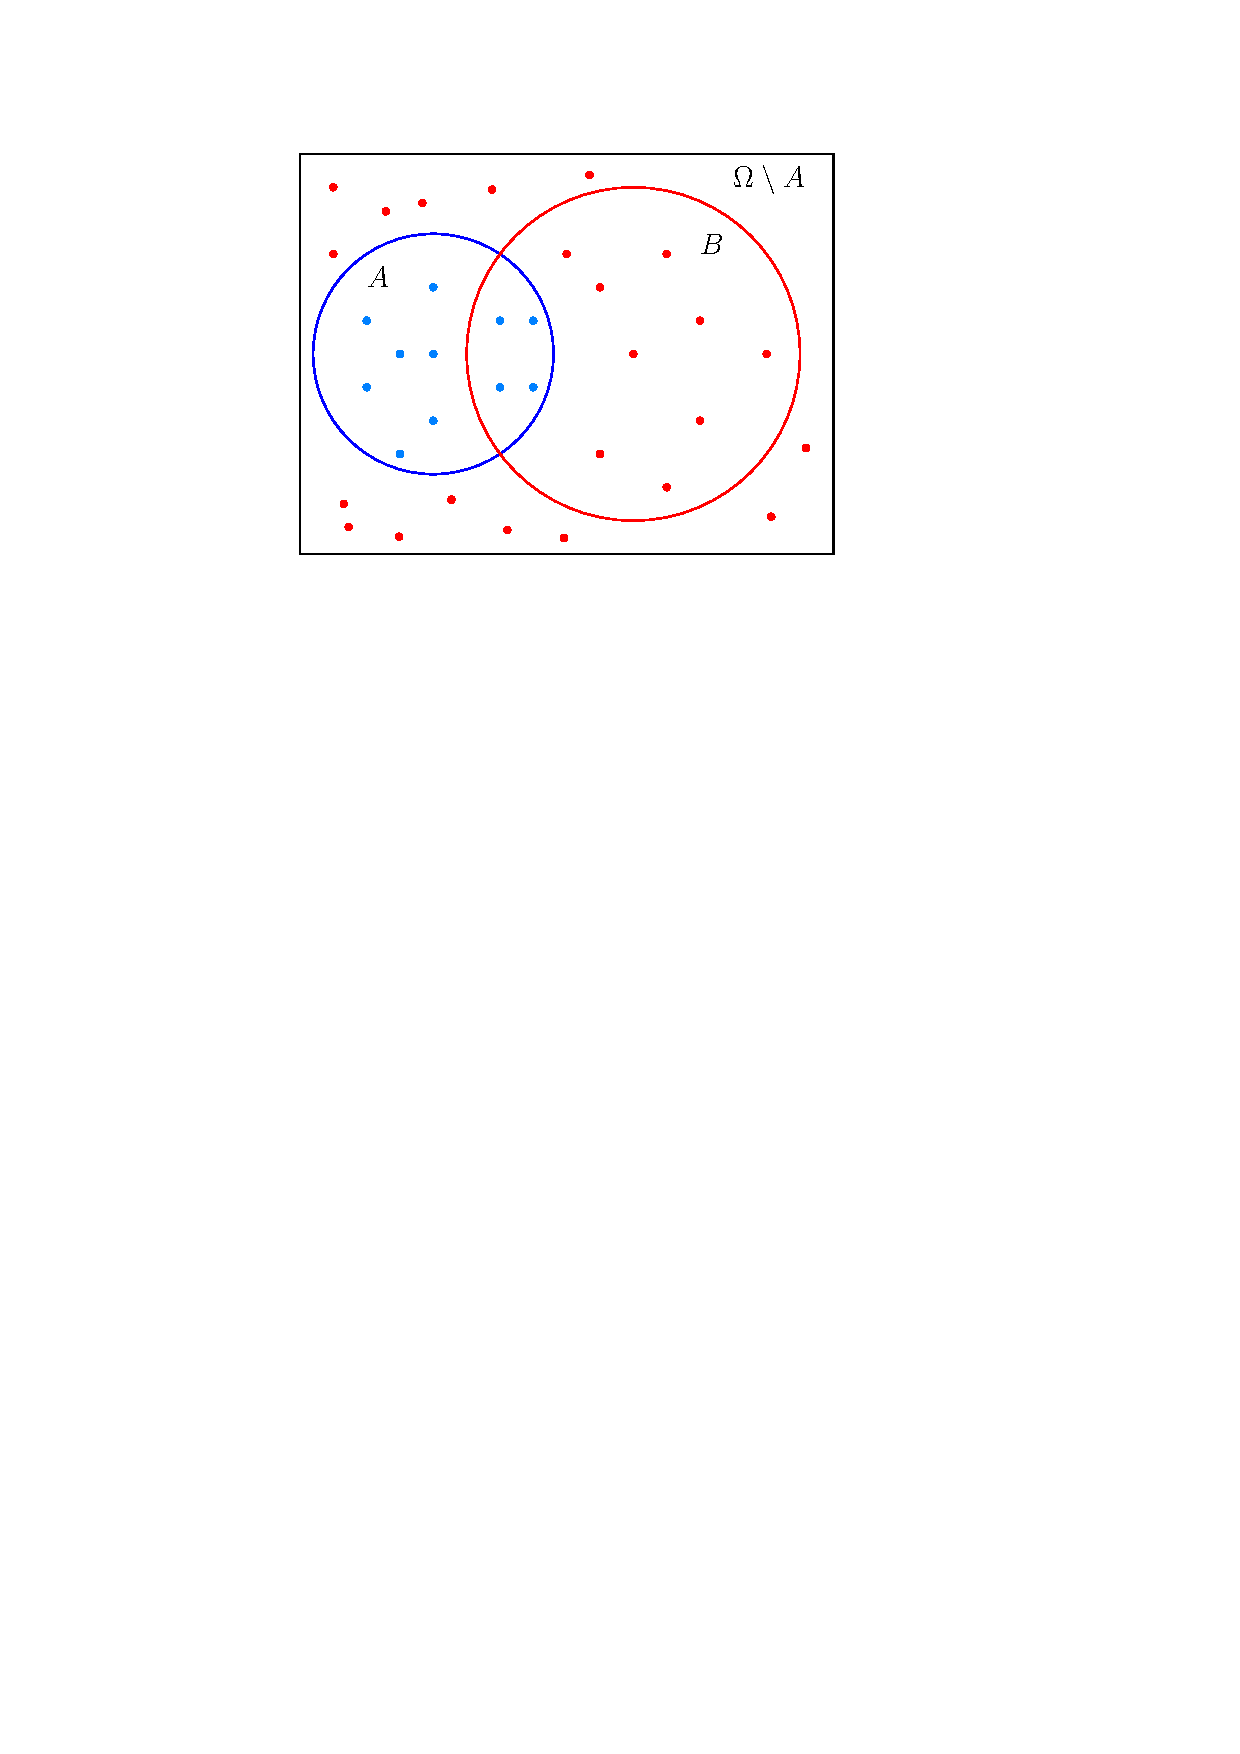
\includegraphics[scale=\normalipe]{ch04_nezavislost_jevu.pdf}
    \caption{Grafické znázornění nezávislosti jevů.}
    \label{fig:nezavislost_jevu}
\end{figure}
Na obrázku \ref{fig:nezavislost_jevu} lze vidět grafické znázornění k vysvětlení výše. Poměr počtu červeně vyznačených elementárních jevů, které náleží jevu $B$ a počtu elementárních jevů, které mu nenáleží, ale náleží $\Omega\setminus A$, je stejný, jako poměr počtu elementárních jevů, které náleží $A$, ale nikoliv $B$, a počtu elementárních jevů, které náleží $A\cap B$. Protože všechny elementární jevy jsou stejně pravděpodobné, pak příslušné poměry přímo odpovídají daným pravděpodobnostem. tzn.
\[\dfrac{\sizeof{A\cap B}}{\sizeof{A}}=\dfrac{\sizeof{B\setminus A}}{\sizeof{\Omega\setminus A}}\]
\begin{task}
    Házíme $n$-krát spravedlivou mincí. Jaká pravděpodobnost, že 2-krát za sebou padne líc?
\end{task}
\begin{solution}
    První hod mince jistě nijak neovlivní druhý hod. Protože házíme dvakrát, množinu elementárních jevů nyní tvoří uspořádané dvojice, kdy první, resp. druhá souřadnice značí, zda v prvním, resp. druhém hodu padl rub (R) nebo líc (L), tj. $\Omega=\set{(R,\,R),\,(R,\,L),\,(L,\,R),\,(L,\,L)}$. Jev, kdy v prvním hodu padl líc, si označíme $A=\set{(L,\,R),\,(L,\,L)}$, a jev, kdy padl v druhém hodu líc, si označíme $B=\set{(R,\,L),\,(L,\,L)}$. Protože nás zajímá, kdy padne v obou hodech líc, pak nás zajímá jev $A\cap B=\set{(L,\,L)}$. Tedy pravděpodobnost, že tento jev nastane, je
    \[\Prob(A\cap B)=\dfrac{\sizeof{A\cap B}}{\sizeof{\Omega}}=\dfrac{1}{4}=25\,\%.\]
    Avšak, jak se můžeme přesvědčit, platí také
    \[\Prob(A\cap B)=\Prob(A)\cdot\Prob(B)=\dfrac{1}{2}\cdot\dfrac{1}{2}=\dfrac{1}{4}.\]
    Jevy $A$ a $B$ jsou tedy \textbf{nezávislé}.
\end{solution}
Jedna věc se zde může zdát zarážející. Pokud se ohlédneme zpět za definicí nezávislých jevů \ref{def:nezavisle_jevy}, můžeme si všimnout, že ačkoliv nám definice dává v podstatě "návod", jak počítat pravděpodobnost nezávislých jevů, přesto jsme se u příkladu výše byly "nuceni" uchýlit ke klasickému výpočtu pravděpodobnosti z definice, tj. \emph{počet příznivých možností ke počtu všech možných možností}, a to proto, že jsme dopředu nevěděli, zda uvažované jevy jsou skutečně nezávislé a museli jsme tuto skutečnost ověřit výpočtem. Nezdá se, že tak naše definice byla něčemu užitečná. Ale není tomu tak, neboť si stačí uvědomit následující věc. Představme si, že máme množinu elementárních jevů $\Omega=\set{\omega_1,\,\omega_2,\,\dots,\,\omega_n}$ a libovolné disjunktní jevy $A,\,B\subseteq\Omega$. Uvažme, že chceme vypočítat pravděpodobnost, že při dvou pokusech nejdříve nastane jev $A$ a pak jev $B$. Pak tuto pravděpodobnost lze stanovit právě pomocí vzorce
\[\Prob(A\cap B)=\Prob(A)\cdot\Prob(B).\]
Je tomu tak z důvodu, že pokud provádíme dva pokusy, pak množina všech možných jevů, označme $\Omega^\prime$, obsahuje uspořádané dvojice (jako u úlohy s hodem mincí), tj. $\Omega^\prime=\set{(\omega_i,\,\omega_j)\admid 0\leqslant i,\,j\leqslant n}$ (tedy zde započítáváme i kolik pokusů provádíme; obecně pokud bychom prováděli $k$ pokusů, pak tato množiny bude obsahovat uspořádané $k$-tice). Tzn. jev $A\cap B$ obsahuje všechny dvojice, které náleží jak jevu $A$, tak jevu $B$, tj. takové, které na příslušných souřadnicích mají elementární jevy z $A$ a $B$. Formálně zapsáno:
\[A\cap B=\set{(\varphi,\,\psi)\admid\varphi\in A \land \psi\in B}.\]
Chceme nyní vypočítat $\Prob(A\cap B)$. K tomu potřebujeme znát $\sizeof{A\cap B}$ a $\sizeof{\Omega^\prime}$. Protože víme, že $\sizeof{\Omega}=n$ a $\Omega^\prime$ je množina všech uspořádaných dvojic z elementárních jevů $\Omega$, pak $\sizeof{\Omega^\prime}=n^2$.\par
Velikost průniku $A\cap B$ lze určit následující úvahou. Pokud elementární jevy jevu $A$ obsahují na první souřadnici elementární jevy množiny $\Omega$, které si označíme
\[\varphi_1,\,\varphi_2,\,\dots,\,\varphi_m,\]
pak $\sizeof{A}=mn$. Analogicky pro obsahující uspořádané dvojice, kde na druhé souřadnici jsou elementární jevy
\[\psi_1,\,\psi_2,\,\dots,\,\psi_k,\]
je $\sizeof{B}=kn$. Tedy pravděpodobnost, že nastane jev $A$, je tak
\[\Prob(A)=\dfrac{\sizeof{A}}{\sizeof{\Omega}}=\dfrac{mn}{n^2}=\dfrac{m}{n}\]
a analogicky pro $B$ je pravděpodobnost
\[\Prob(B)=\dfrac{\sizeof{B}}{\sizeof{\Omega}}=\dfrac{kn}{n^2}=\dfrac{k}{n}.\]
\begin{figure}[H]
    \centering
    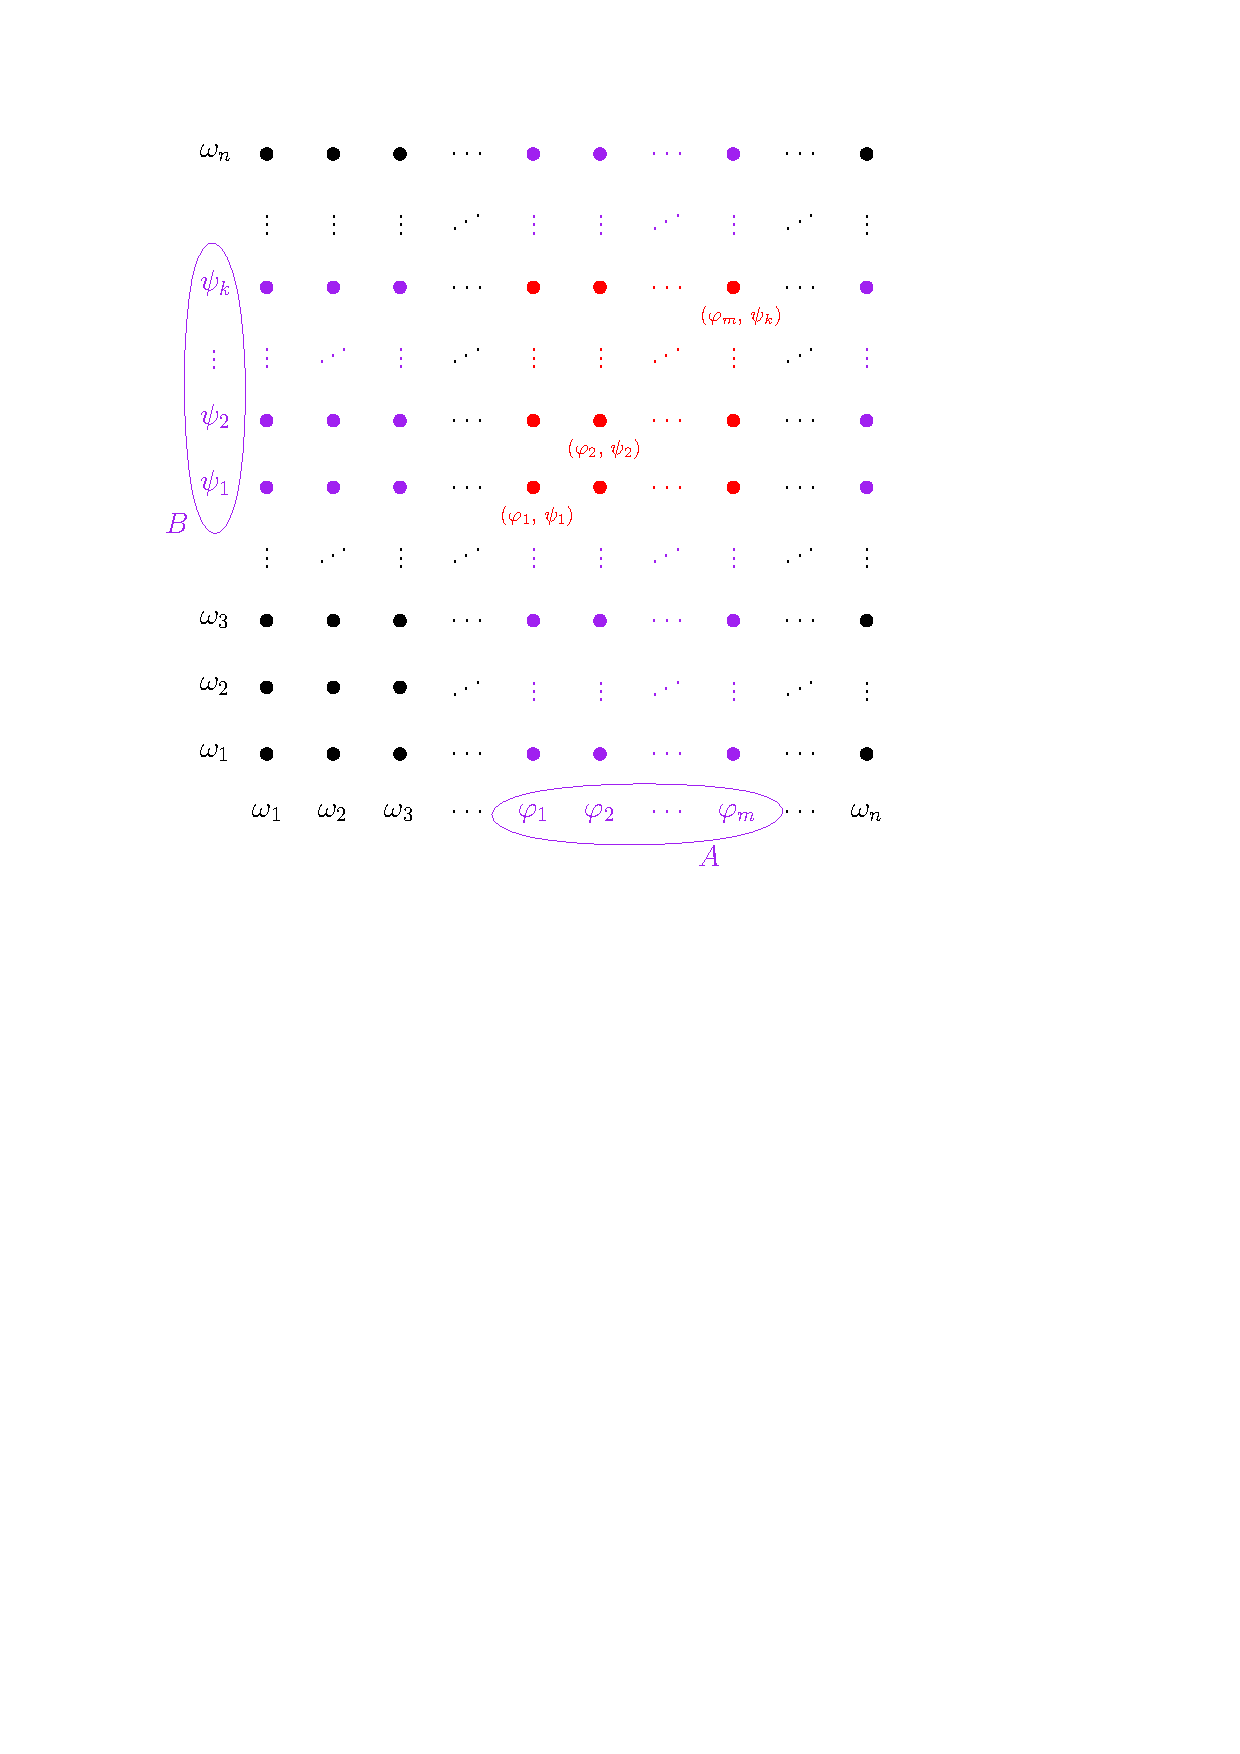
\includegraphics[scale=\normalipe]{ch04_dvojice_podil.pdf}
    \caption{Znázornění jevů $A$ a $B$ v množině $\Omega^\prime$.}
    \label{fig:dvojice_podil}
\end{figure}
Nakonec velikost průniku jevů $A$ a $B$ je $mk$ (viz obrázek \ref{fig:dvojice_podil}). Nyní již můžeme určit pravděpodobnost jevu $A\cap B$, tedy
\[\Prob(A\cap B)=\dfrac{\sizeof{A\cap B}}{\sizeof{\Omega^\prime}}=\dfrac{mk}{n^2}=\dfrac{m}{n}\cdot\dfrac{k}{n}=\Prob(A)\cdot\Prob(B).\]
Tedy jevy $A$ a $B$ jsou skutečně nezávislé. Při obecnější úvaze bychom mohli uvažovat jevy $A$ a $B$ jako podmnožiny dvou různých množin elementárních jevů a došli bychom ke stejnému výsledku. (Zkuste si rozmyslet.)
\medskip

Nyní se podíváme na několik dalších příkladů využití nezávislosti jevů. Aktuálně jsme si již vysvětlili formální pozadí teorie pravděpodobnosti a to především, abychom jsme si vybudovali určitý způsob chápání náhody v řeči matematiky. Zatím jsme tak v rámci formalizace při řešení různých úloh kromě samotného výpočtu řešili také určení množiny elementárních jevů, abychom naši jinak abstraktní definici ukázali v aplikaci na konkrétních příkladech. Nicméně pokud se podíváte na úlohy v různých sbírkách (hlavně na internetu) na pravděpodobnost, jen málokde byste v jejich řešení našly tyto kroky a zejména z důvodu, že tyto záležitosti jsou považovány za intuitivní. Abychom se vyhnuli zdlouhavým řešením a jejich zápisům, budeme řešení provádět od teď o něco stručněji.
\begin{task}
    Ve městě jsou čtyři křižovatky se světelnými semafory. Každý z nich uvolňuje nebo uzavírá dopravu se stejnou pravděpodobností $0{,}5$. Jaká je pravděpodobnost, že auto:
    \begin{enumerate}[label=(\alph*)]
        \item projde první křižovatkou bez zdržení,
        \item projde prvními dvěma křižovatkami bez zdržení,
        \item projde všemi čtyřmi křižovatkami bez zdržení.
    \end{enumerate}
\end{task}
\begin{solution}
    Každá z těchto křižovatek představuje \emph{samostatnou situaci}, kde chceme spočítat, zda auto projede, nebo neprojede bez zdržení. Všechny situace, kdy auto projede bez zdržení tak u každé křižovatky tvoří samostatný jev\footnote{Technicky vzato zde máme 4 množiny elementárních jevů pro každou křižovatku, ale předešlou úvahu o nezávislých jevech lze aplikovat i pro různé množiny elementárních jevů (tj. nemusí být nutně stejné).}, tj. $K_1,\,K_2,\,K_3,\,K_4$, které jsou nezávislé. Body \textit{(a)}, \textit{(b)} a \textit{(c)} tak vyřešíme následovně:
    \begin{enumerate}[label=(\alph*)]
        \item $\displaystyle \Prob(K_1)=0{,}5=50\,\%$,
        \item $\displaystyle \Prob(K_1\cap K_2)=0{,}5\cdot 0{,}5=0{,}25=25\,\%$,
        \item $\displaystyle \Prob(K_1\cap K_2\cap K_3)=0{,}5\cdot 0{,}5\cdot 0{,}5=0{,}125=12{,}5\,\%.$
    \end{enumerate}
\end{solution}
\begin{task}
    Máme falešnou kostku, kde čísla padají s pravděpodobnostmi.
    \begin{itemize}
        \item $\Prob(\set{1})=0{,}1$;
        \item $\Prob(\set{2})=0{,}2$;
        \item $\Prob(\set{3})=0{,}22$;
        \item $\Prob(\set{4})=0{,}16$;
        \item $\Prob(\set{5})=0{,}24$;
        \item $\Prob(\set{6})=0{,}08$.
    \end{itemize}
    Určete pravděpodobnost, že při dvou hodech padnou stejná čísla. \citep[příklad \textit{Falešná kostka
    }]{hackmath2022}
\end{task}
\begin{solution}
    Každý hod kostkou tvoří nezávislý jev, tedy pravděpodobnost, že dvakrát za sebou padne stejné číslo $i$ (označme $D_i$) je rovna
    \[\Prob(D_i)=\Prob(\set{i})\cdot\Prob(\set{i})=\Prob(\set{i})^2.\]
    Pro všechna různá $i,\,j$ jsou však jevy $D_i$ a $D_j$ disjunktní (nemůže nám padnout dvakrát za sebou číslo $i$ a zároveň dvakrát za sebou číslo $j$). Tedy výsledná pravděpodobnost je
    \begin{align*}
        \Prob\left(\bigcup\limits_{i=1}^{6}D_i\right)&=\sum_{i=1}^{6}\Prob(D_i)=\sum_{i=1}^{6}\Prob(\set{i})^2\\
        &=0{,}1^2+0{,}2^2+0{,}22^2+0{,}16^2+0{,}24^2+0{,}08^2=0{,}188=18{,}8\,\%.
    \end{align*}
\end{solution}
\begin{task}
    \textit{Kolikrát musíme hodit mincí, aby pravděpodobnost, že padne alespoň jednou líc byla větší než $0{,}999$?} \citep[str. 171]{Petakova2020}
\end{task}
\begin{solution}
    Máme spravedlivou minci, tedy pravděpodobnost, že padne líc je $1/2$. Zkusíme úlohu vyřešit opačným způsobem, tedy vypočítáme pravděpodobnost obecně pro $n$ pokusů, že nepadl ani jednou líc (což je jev opačný k jevu, který máme vyšetřit). To znamená, že řešíme pravděpodobnost jevu, že $n$-krát po sobě padl rub. Označme si jev, kdy po $n$ pokusech padl alespoň jednou líc, jako $L$. Tzn. jev, kdy padne $n$-krát po sobě rub, je $L^\complement$. Pravděpodobnost jevu $L^\complement$ je tak
    \[\Prob\left(L^\complement\right)=\left(\dfrac{1}{2}\right)^n.\]
    Tedy pravděpodobnost jevu $L$ je
    \[\Prob(L)=1-\left(\dfrac{1}{2}\right)^n,\]
    přičemž nás zajímá, pro jaké $n$ tato pravděpodobnost přesáhne hodnotu $0{,}999$. Tedy řešíme nerovnici
    \begin{align*}
        1-\left(\dfrac{1}{2}\right)^n&\geqslant 0{,}999\\
        0{,}001&\geqslant\left(\dfrac{1}{2}\right)^n\\
        \dfrac{1}{1000}&\geqslant\dfrac{1}{2^n}\\
        2^n&\geqslant 1000\\
        n&\geqslant\log_2{1000}\approx 9{,}966\\
        n&\geqslant 10.
    \end{align*}
    Tedy pro $n\geqslant 10$ pravděpodobnost, že padne alespoň jednou líc, přesáhne hodnotu $0{,}999$.
\end{solution}
    \chapwithtoc{Výsledky cvičení}

\textbf{\ref{exercise:ch02_1}}\quad 15 způsobů.\\
\textbf{\ref{exercise:ch02_2}}\quad 34 žáků.\\
\textbf{\ref{exercise:ch02_3}}\quad 216 čísel.\\
\textbf{\ref{exercise:ch02_4}}\quad 336 způsobů.\\
\textbf{\ref{exercise:ch02_5}}\quad $30!/2$\\
\textbf{\ref{exercise:ch02_6}}\quad 44.\\
\textbf{\ref{exercise:ch02_7}}\quad $32!$ způsobů.\\
\textbf{\ref{exercise:ch02_8}}\quad 362800 čísel.\\
\textbf{\ref{exercise:ch02_9}}\quad (a) 45 přímek; (b) 31 přímek.\\
\textbf{\ref{exercise:ch02_10}}\quad $n(n-3)/2$.\\
\textbf{\ref{exercise:ch02_11}}\quad (a) 50 388; (b) 75 582; (c) 18 564; (d) 43 758.\\
\textbf{\ref{exercise:ch02_12}}\quad 45.\\
\textbf{\ref{exercise:ch02_13}}\quad 24 způsobů.\\

    % Bibliography
    
    \renewcommand{\bibname}{Seznam použité literatury}

    % \bibliographystyle{plainnat}    %% Autor (rok) s anglickými spojkami
    \bibliographystyle{unsrtnat}       %% [číslo]
    % \bibliographystyle{alpha}

    %%% Vytvoření seznamu literatury. Pozor, pokud jste necitovali ani jednu
    %%% položku, seznam se automaticky vynechá.
    \bibliography{components/bibliography.bib}

\end{document}